\documentclass{beamer}

\usetheme{AnnArbor}
\setbeamertemplate{footline} {
  % \leavevmode%
  \hbox{%
    \begin{beamercolorbox}[wd=.33\paperwidth,ht=2.25ex,dp=1ex,center]{author in head/foot}%
      \usebeamerfont{author in head/foot}\hspace*{2ex}\insertshortauthor %~(UHH)
    \end{beamercolorbox}%
    \begin{beamercolorbox}[wd=.34\paperwidth,ht=2.25ex,dp=1ex,center]{title
        in head/foot}%
      \usebeamerfont{title in head/foot}\insertshorttitle
    \end{beamercolorbox}%
    \begin{beamercolorbox}[wd=.33\paperwidth,ht=2.25ex,dp=1ex,center]{date in head/foot}%
      \usebeamerfont{date in head/foot}\insertshortdate\hspace*{2ex}
   \end{beamercolorbox}}%
  \vskip0pt%
}
\beamertemplatenavigationsymbolsempty

\usepackage{amsmath}
\usepackage{booktabs}
\usepackage[german]{babel}
\usepackage{graphicx}
\usepackage{rotating}
\usepackage{xspace}


% New commands
\newcommand{\tev}{\ensuremath{\;\text{Te}\kern-0.06667em\text{V}}\xspace}
\newcommand{\gev}{\ensuremath{\;\text{Ge}\kern-0.06667em\text{V}}\xspace}
\newcommand{\mev}{\ensuremath{\;\text{Me}\kern-0.06667em\text{V}}\xspace}
\newcommand{\kev}{\ensuremath{\;\text{ke}\kern-0.06667em\text{V}}\xspace}
\newcommand{\ev}{\ensuremath{\;\text{e}\kern-0.06667em\text{V}}\xspace}
\newcommand{\km}{\ensuremath{\;\text{km}}\xspace}
\newcommand{\m}{\ensuremath{\;\text{m}}\xspace}
\newcommand{\cm}{\ensuremath{\;\text{cm}}\xspace}
\newcommand{\mm}{\ensuremath{\;\text{mm}}\xspace}
\newcommand{\hour}{\ensuremath{\;\text{h}}\xspace}
\newcommand{\second}{\ensuremath{\;\text{s}}\xspace}
\newcommand{\kg}{\ensuremath{\;\text{kg}}\xspace}
\newcommand{\tons}{\ensuremath{\;\text{t}}\xspace}
\newcommand{\tesla}{\ensuremath{\;\text{T}}\xspace}
\newcommand{\kelvin}{\ensuremath{\;\text{K}}\xspace}
\newcommand{\nbinv}{\ensuremath{\;\text{nb}^{-1}}\xspace}
\newcommand{\pbinv}{\ensuremath{\;\text{pb}^{-1}}\xspace}
\newcommand{\fbinv}{\ensuremath{\;\text{fb}^{-1}}\xspace}
\newcommand{\znull}{\ensuremath{Z^{0}}\xspace}
\newcommand{\ca}{ca.\ }
\newcommand{\zb}{z.\,B.\ }


\graphicspath{{../CommonGraphics/}}


% Title etc
\title[Masterclass Teilchenphysik]{Die Bausteine des Universums}
\subtitle{Masterclass Teilchenphysik --- Heinrich-Heine-Gymnasium Hamburg}
\author[D. Britzger, H. Kirschenmann]{Daniel Britzger, Henning Kirschenmann}
\institute[Universit\"at Hamburg]{}
\date[7. August 2013]{7. August 2013}
\titlegraphic{
\vskip1cm

\includegraphics[height=1.2cm]{logo/logo-tw-4c}
\hskip1cm

\includegraphics[height=1.2cm]{logo/UHH-Logo_2010_Farbe_CMYK}
\hskip1cm

\includegraphics[height=1.2cm]{logo/DESY-Logo-cyan-RGB_mitVorschau_ger}}

% pdflatex packages
\hypersetup{bookmarks=true}
\hypersetup{unicode=true}
\hypersetup{pdftitle={Masterclass Teilchenphysik}}
\hypersetup{pdfauthor={Matthias Schr\"oder}}
\hypersetup{bookmarks=true}


\begin{document}
% ==================================================
\begin{frame}
  \titlepage
\end{frame}


% ==================================================
\section{Einleitung}
% --------------------------------------------------
{\usebackgroundtemplate{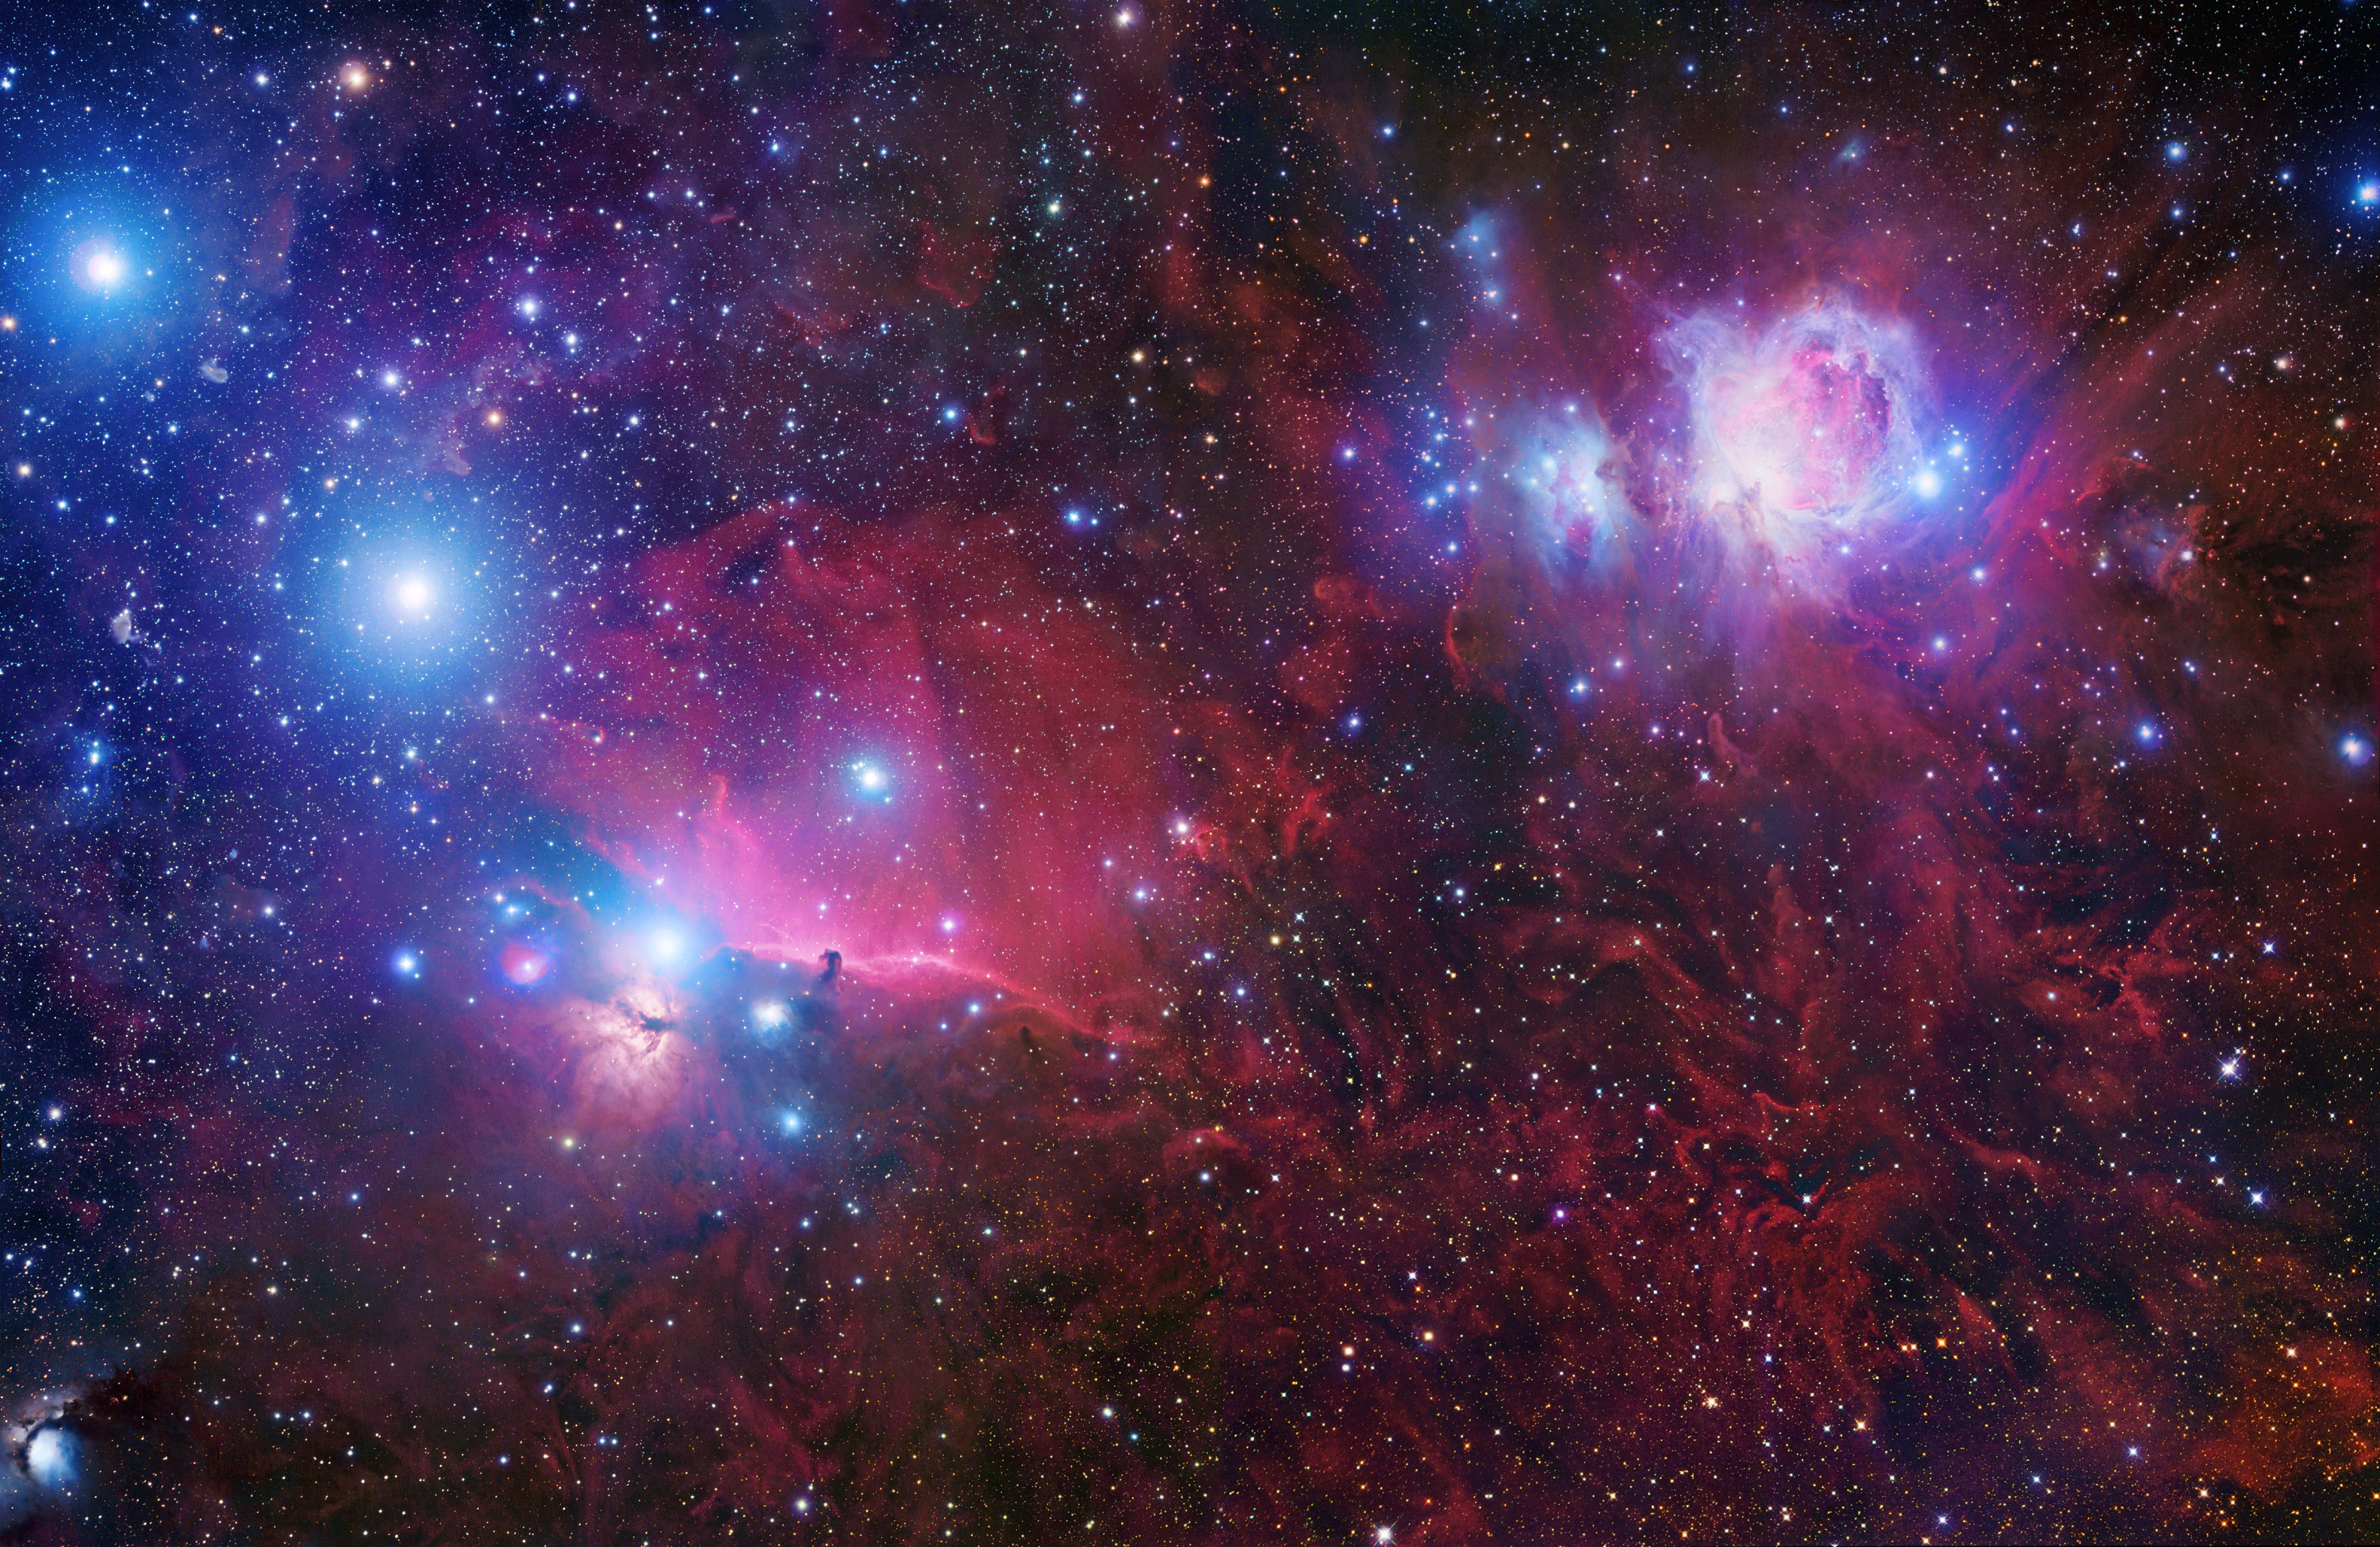
\includegraphics[height=\paperheight]{cosmology/oriondeepwide_gendler_f.jpg}}
  
  % --------------------------------------------------
  \begin{frame}
    \begin{center}
      \visible<3->{\textcolor{white}{\Large Teilchenphysik}}
      \vskip0.3cm
      \visible<3->{\textcolor{white}{\Large stellt}}
      \vskip0.4cm
      \visible<2->{\textcolor{white}{\Huge FRAGEN}}
    \end{center}
  \end{frame}

  \subsection{Fragen der Teilchenphysik}  
  % --------------------------------------------------
  \begin{frame}[t]
    \frametitle{Fragen der Teilchenphysik}
    \vskip0.5cm
    \begin{itemize}
    \item[~]<2-> \textcolor{white}{Woraus besteht das Universum? Woraus bestehen wir?}
      \begin{itemize}
      \item[~]<2-> \textcolor{white}{Grundbausteine der Materie}
      \end{itemize}
    \item[~]<3-> \textcolor{white}{Wie funktioniert das Universum?}
      \begin{itemize}
      \item[~]<3-> \textcolor{white}{Wechselwirkungen}
      \end{itemize}
    \item[~]<4-> \textcolor{white}{Wie ist das Universum entstanden?}
      \begin{itemize}
      \item[~]<4-> \textcolor{white}{Zeitliche Entwicklung}
      \end{itemize}
    \end{itemize}
    \only<2>{
      \begin{center}
        \vskip-1cm
        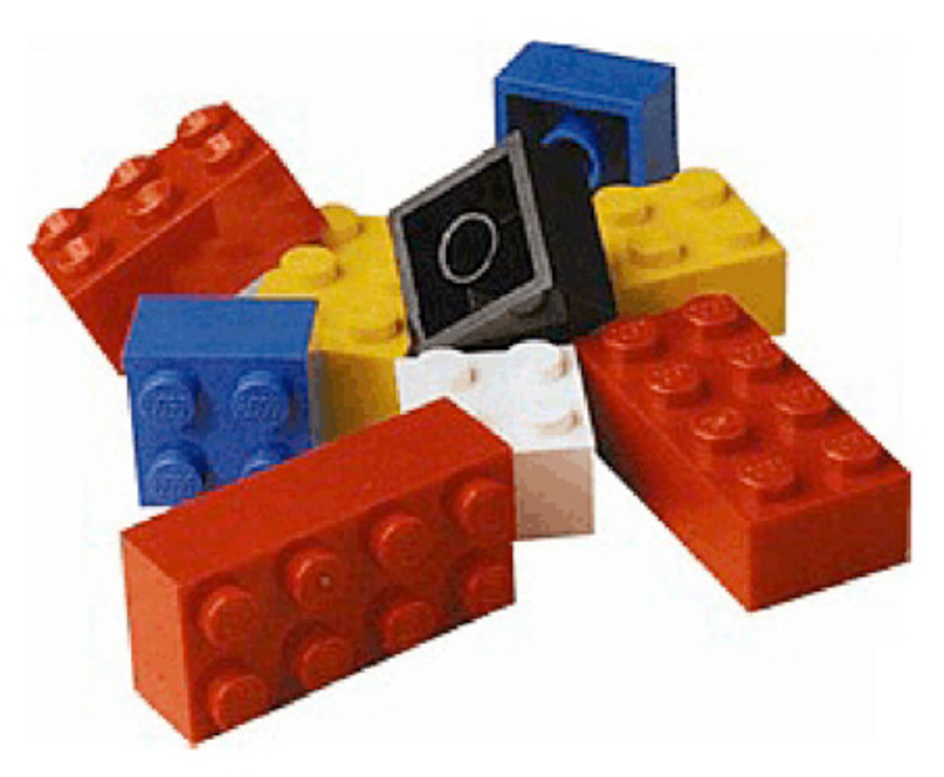
\includegraphics[width=0.4\textwidth]{eyecandy/LEGO-Bricks.pdf}
      \end{center}
    }
    \only<3>{
      \vskip-0.2cm
      \begin{columns}
        \begin{column}{0.3\textwidth}
          \centering
          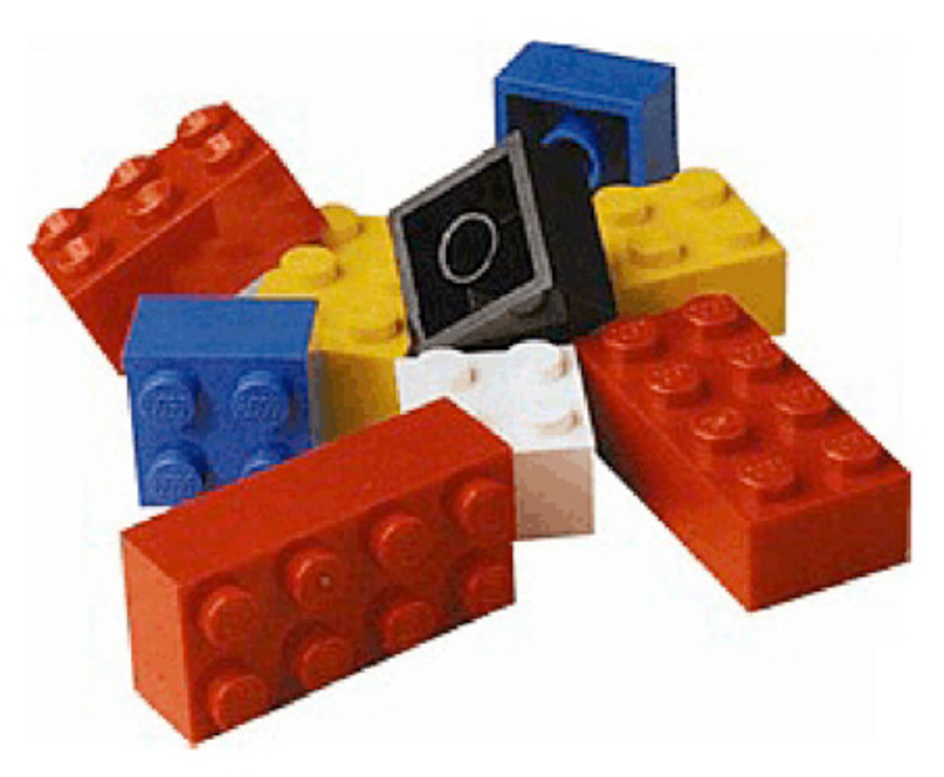
\includegraphics[width=0.8\textwidth]{eyecandy/LEGO-Bricks.pdf}
        \end{column}
        \begin{column}{0.025\textwidth}
          \textbf{\textcolor{white}{\Large +}}
        \end{column}
        \begin{column}{0.25\textwidth}
          \centering
          
\includegraphics[width=\textwidth]{eyecandy/Glue.png}
        \end{column}
        \begin{column}{0.025\textwidth}
          \textbf{\textcolor{white}{\Large =}}
        \end{column}
        \begin{column}{0.4\textwidth}
          \centering
          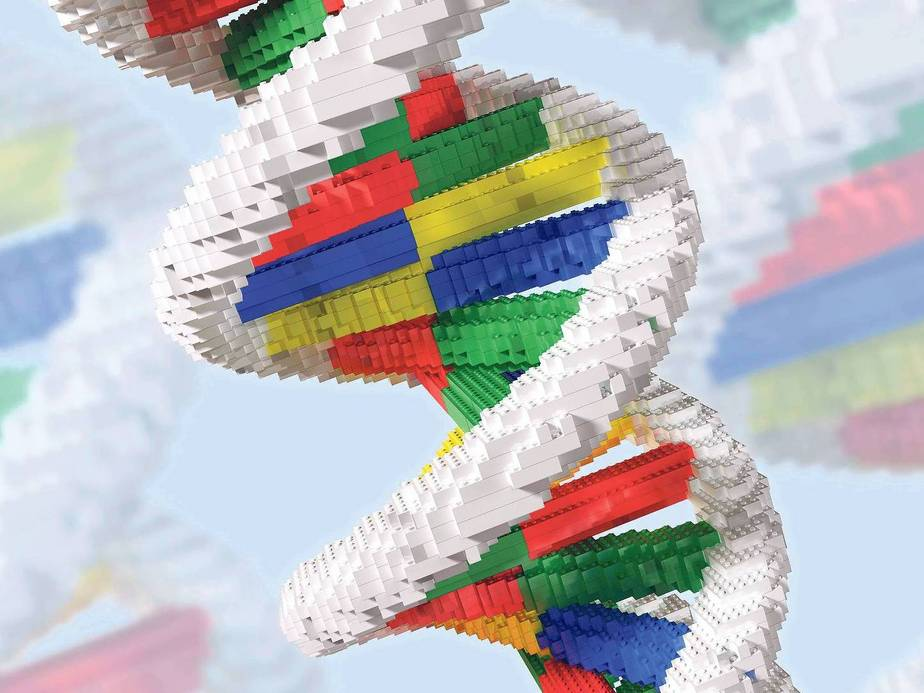
\includegraphics[width=0.9\textwidth]{eyecandy/LEGO-DNS.jpg}
        \end{column}
      \end{columns}
    }
    \only<5->{
      \vskip1cm
      \begin{columns}
        \begin{column}{0.15\textwidth}
        \end{column}
        \begin{column}{0.7\textwidth}
          \begin{block}{}
            \centering \alert{\Large Was sind die fundamentalen
                Bausteine und Kr\"afte im Universum?}
          \end{block}
        \end{column}
        \begin{column}{0.15\textwidth}
        \end{column}
      \end{columns}
    }
  \end{frame}
 
  \subsection{Unser Bild vom Universum}
   % --------------------------------------------------
   \begin{frame}
     \frametitle{Unser Bild vom Universum}
     \begin{center}
       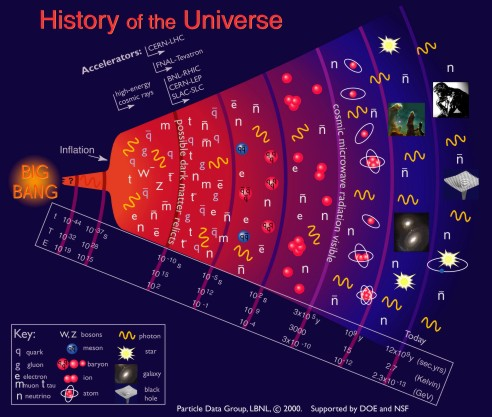
\includegraphics[width=0.7\textwidth]{cosmology/EvolutionOfTheUniverse5.jpg}
     \end{center}
   \end{frame}
   
   % --------------------------------------------------
   \begin{frame}
     \frametitle{Unser Bild vom Universum}
     \begin{center}
       \visible<2->{
         \begin{block}{Rotation von Galaxien}
           \begin{columns}
             \begin{column}{0.35\textwidth}
               \begin{itemize}
               \item Zu wenig sichtbare Materie
               \item<3-> \alert{Dunkle Materie}
               \item[~] ~
               \end{itemize}
             \end{column}
             \begin{column}{0.65\textwidth}
               \centering
               \vskip-0.5cm
               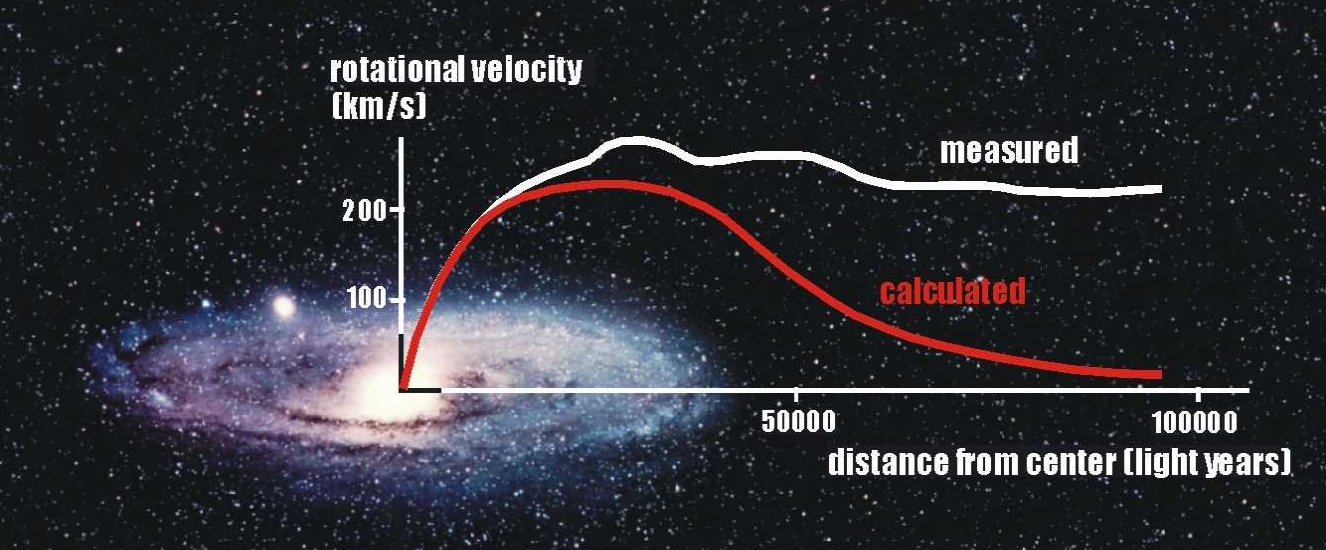
\includegraphics[height=0.35\textheight]{cosmology/DarkMatter_GalaxyRotation.jpg}
             \end{column}
           \end{columns}
         \end{block}
       }
       \visible<4->{
         \begin{block}{Expansion des Universums}
           \begin{columns}
             \begin{column}{0.35\textwidth}
               \begin{itemize}
               \item<5-> Beschleunigte Expansion
               \item<6-> \alert{Dunkle Energie}
               \item[~] ~
               \end{itemize}
             \end{column}
             \begin{column}{0.65\textwidth}
               \centering
               \vskip-0.5cm
               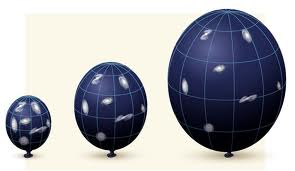
\includegraphics[height=0.35\textheight]{cosmology/UniverseExpansion.jpg}
             \end{column}
           \end{columns}
         \end{block}
       }
     \end{center}
   \end{frame}

   % --------------------------------------------------
   \begin{frame}
     \frametitle{Unser Bild vom Universum}
     \begin{center}
       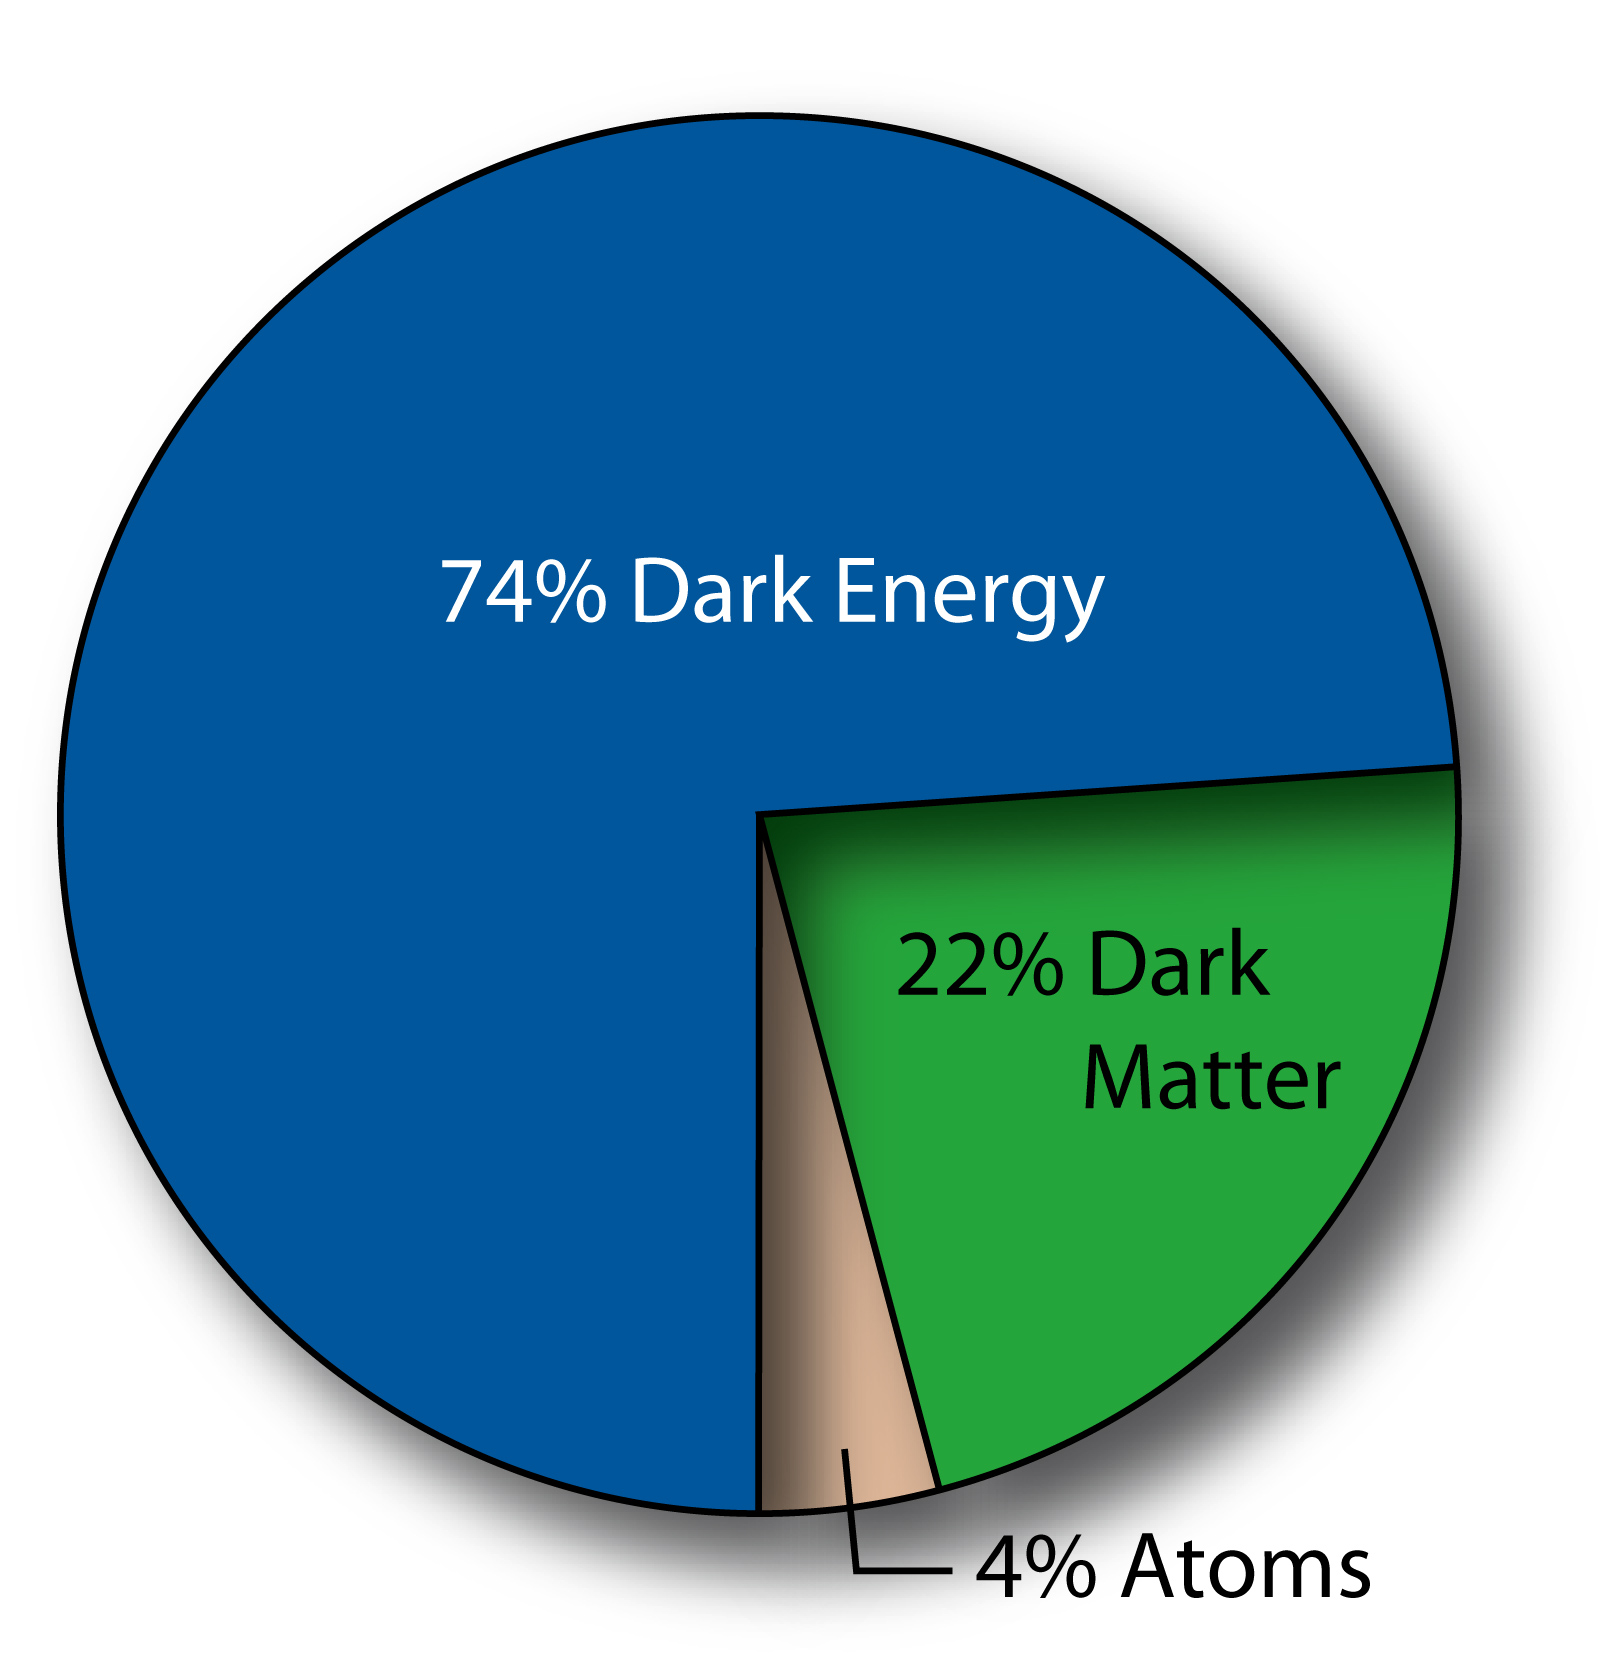
\includegraphics[width=0.45\textwidth]{cosmology/MatterContentOfTheUniverse.jpg}
     \end{center}
     \pause
     \begin{center}
       \begin{block}{}
         \centering
         {\large LHC: \alert{Wir beginnen \textbf{jetzt}, die weiteren $96\%$ zu erforschen!}}
       \end{block}
     \end{center}
   \end{frame}
}

\section{\"Ubersicht}
% --------------------------------------------------
\begin{frame}
  \frametitle{\"Ubersicht}
  \begin{columns}
    \begin{column}{0.05\textwidth}
      \centering
      \alert{\Huge 1}
    \end{column}
    \begin{column}{0.68\textwidth}
      \begin{itemize}
      \item Wie arbeiten Teilchenphysiker?
      \item Was wissen wir \"uber Elementarteilchen?
      \item Was wissen wir \textbf{nicht} \"uber Elementarteilchen?
      \end{itemize}
    \end{column}
    \begin{column}{0.27\textwidth}
      \centering
      \alert{Henning}
    \end{column}
  \end{columns}
  \vskip0.5cm
  \begin{columns}
    \begin{column}{0.05\textwidth}
      \centering
      \alert{\Huge 2}
    \end{column}
    \begin{column}{0.68\textwidth}
      \begin{itemize}
      \item Erforschung von Elementarteilchen
        \begin{itemize}
        \item Wie kann man sie erzeugen?
        \item Wie kann man sie sichtbar machen?
        \end{itemize}
      \end{itemize}
    \end{column}
    \begin{column}{0.27\textwidth}
      \centering
      \alert{Daniel}
    \end{column}
  \end{columns}
  \begin{center}
    ---------------------------------   Mittagspause   ---------------------------------
  \end{center}
  \begin{columns}
    \begin{column}{0.05\textwidth}
      \centering
      \alert{\Huge 3}
    \end{column}
    \begin{column}{0.68\textwidth}
      \begin{itemize}
      \item Selber forschen!
        \begin{itemize}
        \item Wie kann man sie erzeugen?
        \item Wie kann man sie sichtbar machen?
        \end{itemize}
      \end{itemize}
    \end{column}
    \begin{column}{0.27\textwidth}
      \centering
      \alert{Alle zusammen}
    \end{column}
  \end{columns}
\end{frame}

% --------------------------------------------------
\begin{frame}
  \frametitle{Regeln}
  \begin{center}
    {\Huge FRAGEN stellen!}
  \end{center}
\end{frame}

\section{Naturwissenschaftliches Arbeiten}
% --------------------------------------------------
\begin{frame}
  \frametitle{Wie erforscht man denn das Universum?}
  \vskip-0.5cm
  \begin{columns}[T]
    \begin{column}{0.55\textwidth}
      \begin{flushleft}
        oder: Wie arbeiten Teilchenphysiker?
      \end{flushleft}
      \begin{center}
        \only<1-2>{
          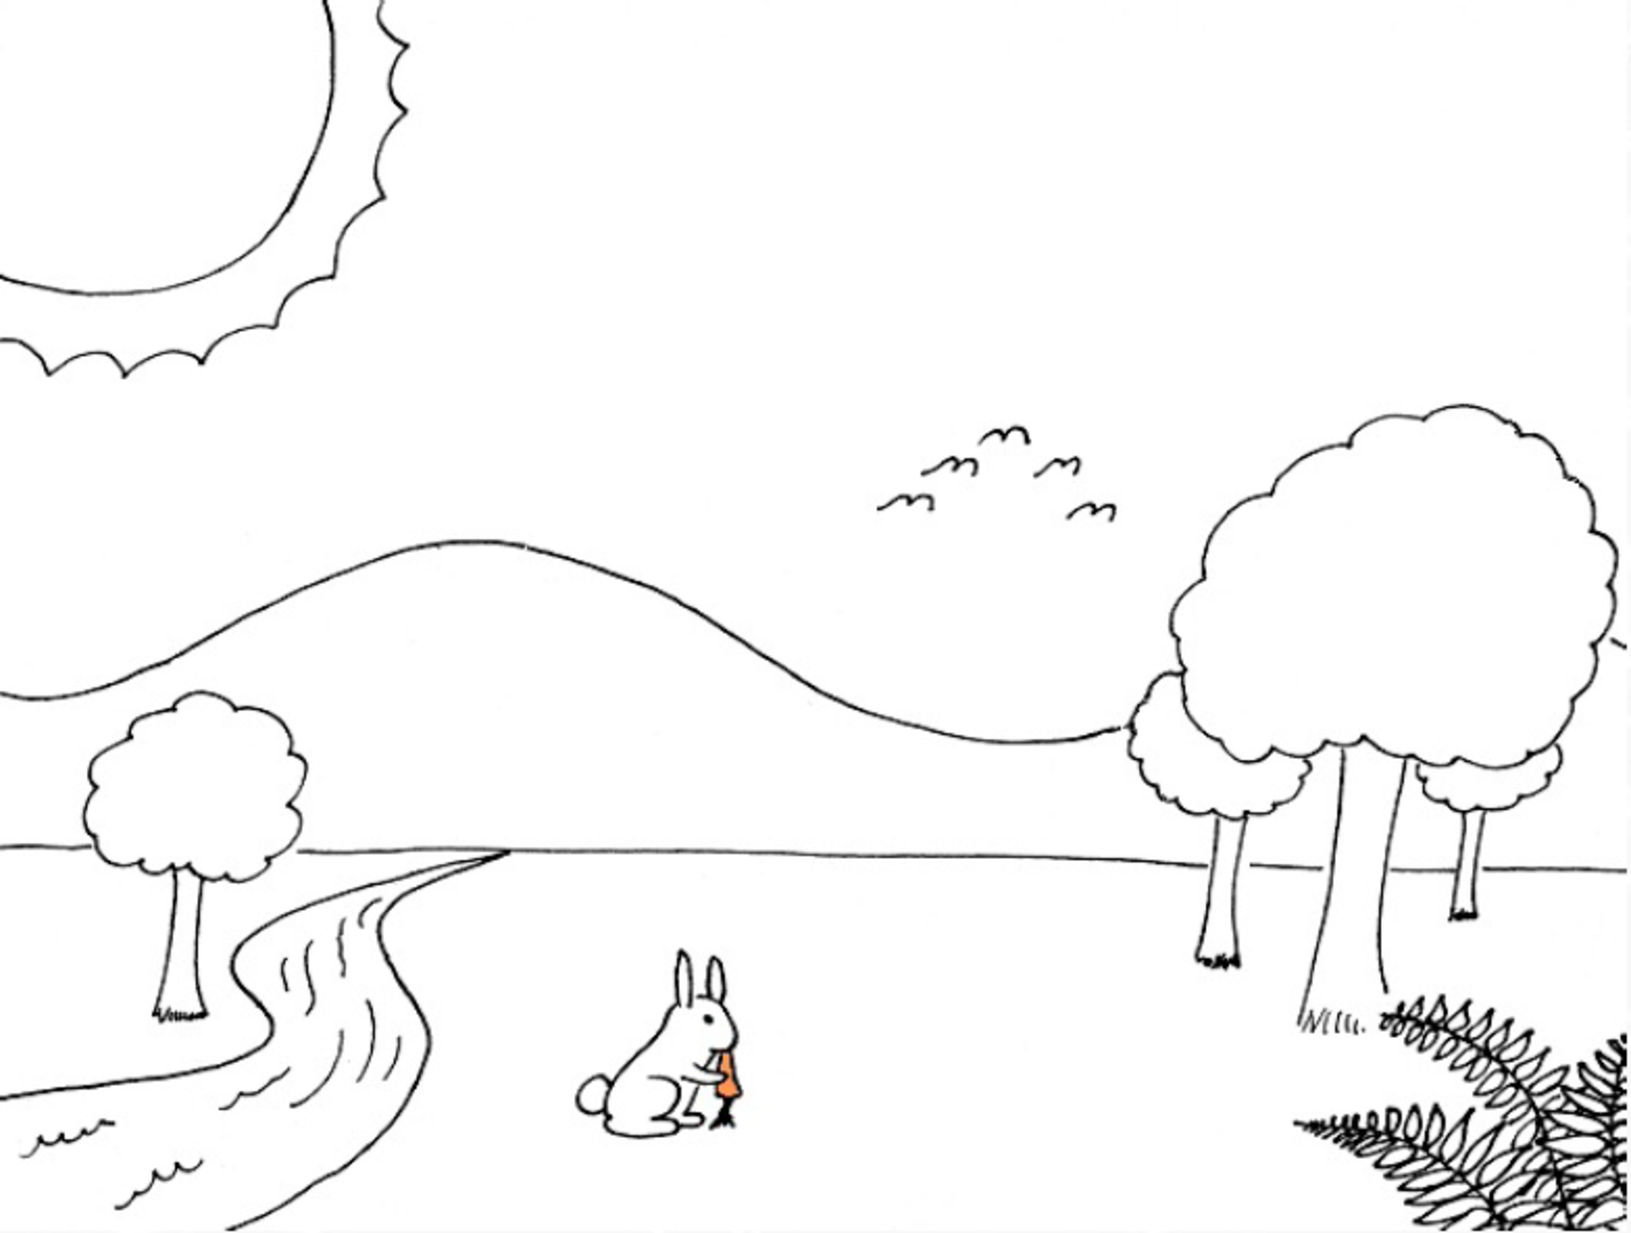
\includegraphics[width=\textwidth]{eyecandy/Wiese.pdf}
        }
        \only<3->{
          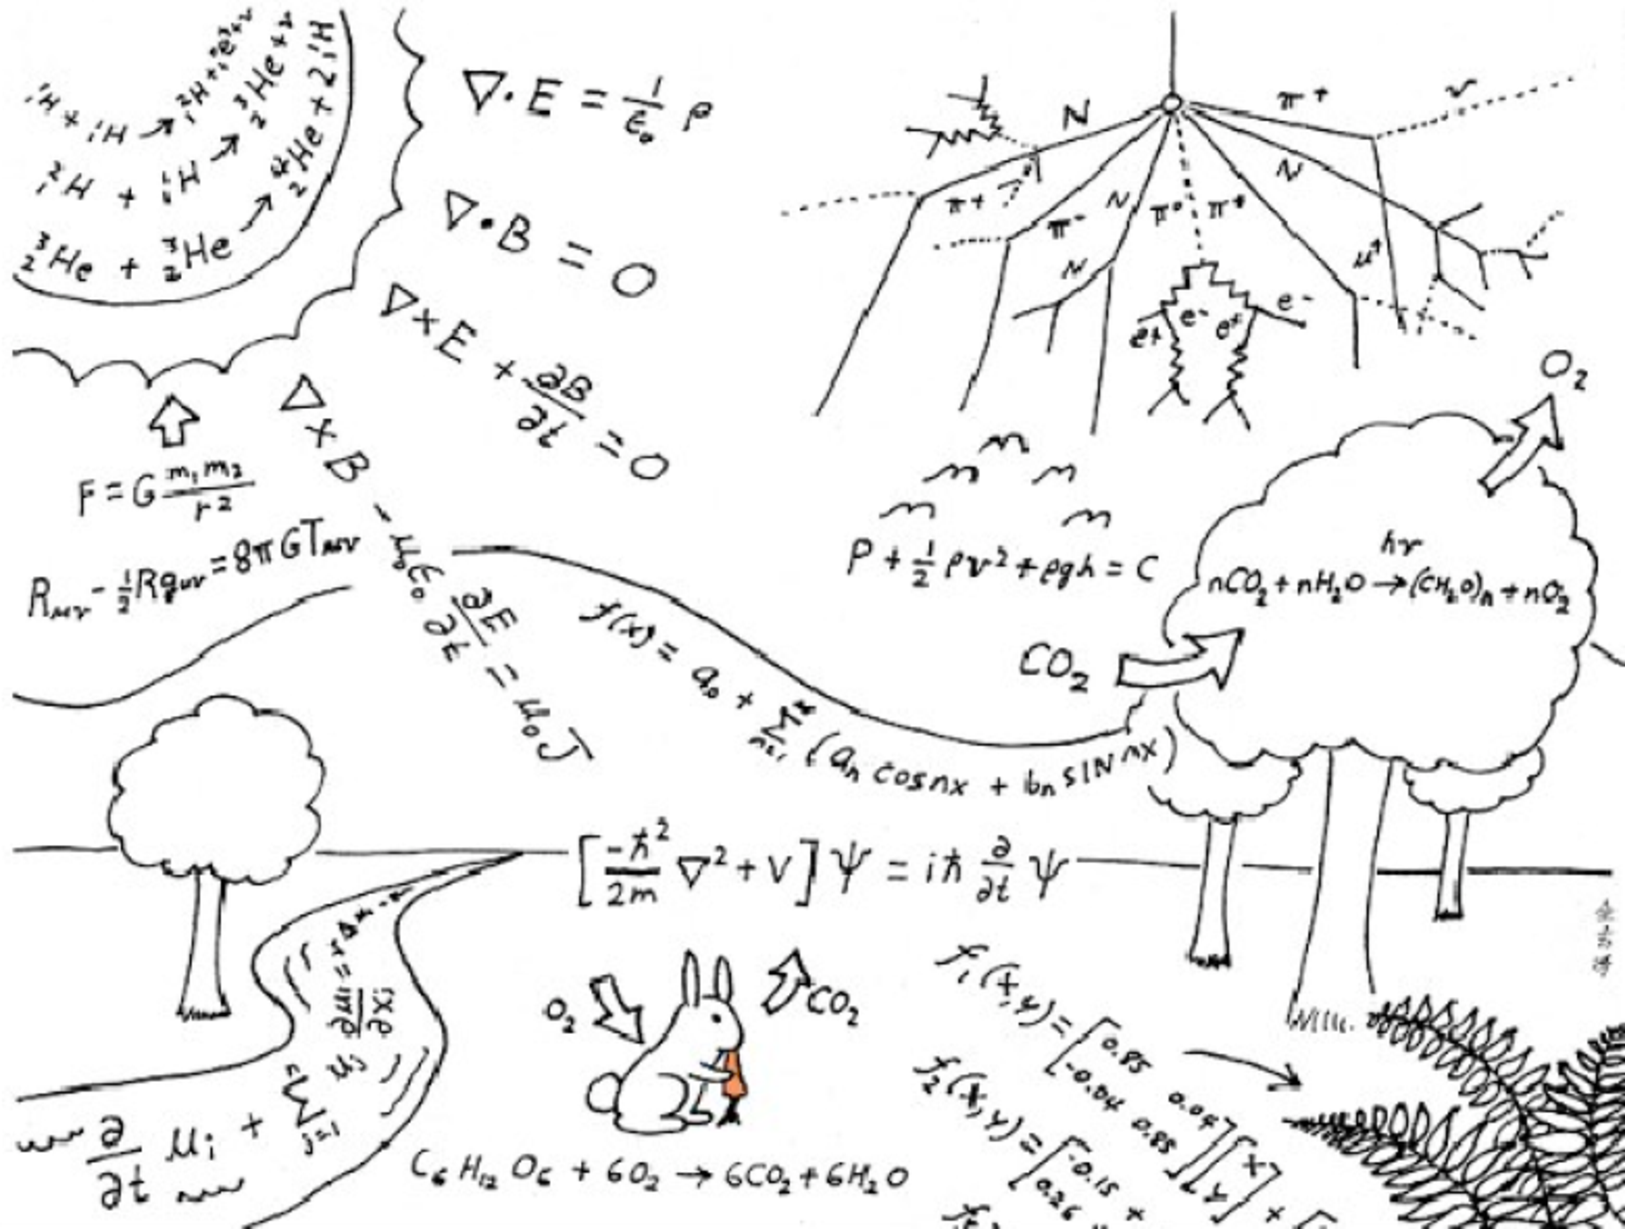
\includegraphics[width=\textwidth]{eyecandy/Wiese-Modell.pdf}
        }
      \end{center}
    \end{column}
    \begin{column}{0.45\textwidth}
      \visible<2->{
        \begin{center}
          \alert{Theoretischer Physiker}\\
        \end{center}
        \begin{center}
          
\includegraphics[height=3cm]{eyecandy/Sheldon}\\
        \end{center}
        \alert{Entwickelt Modelle}
      }
      \visible<3->{
        \begin{itemize}
        \item Mathemat. Formulierung
          \begin{itemize}
          \item z.B. Standardmodell
          \end{itemize}
        \item Wenige Grundannahmen
          \begin{itemize}
          \item z.B. Energieerhaltung
          \end{itemize}
        \end{itemize}
      }
    \end{column}
  \end{columns}
\end{frame}

% --------------------------------------------------
\begin{frame}
  \frametitle{Wie erforscht man denn das Universum?}
  \vskip-0.6cm
  \begin{columns}[T]
    \begin{column}{0.55\textwidth}
      \begin{flushleft}
        oder: Wie arbeiten Teilchenphysiker?
      \end{flushleft}
      \begin{center}
        \only<1>{
          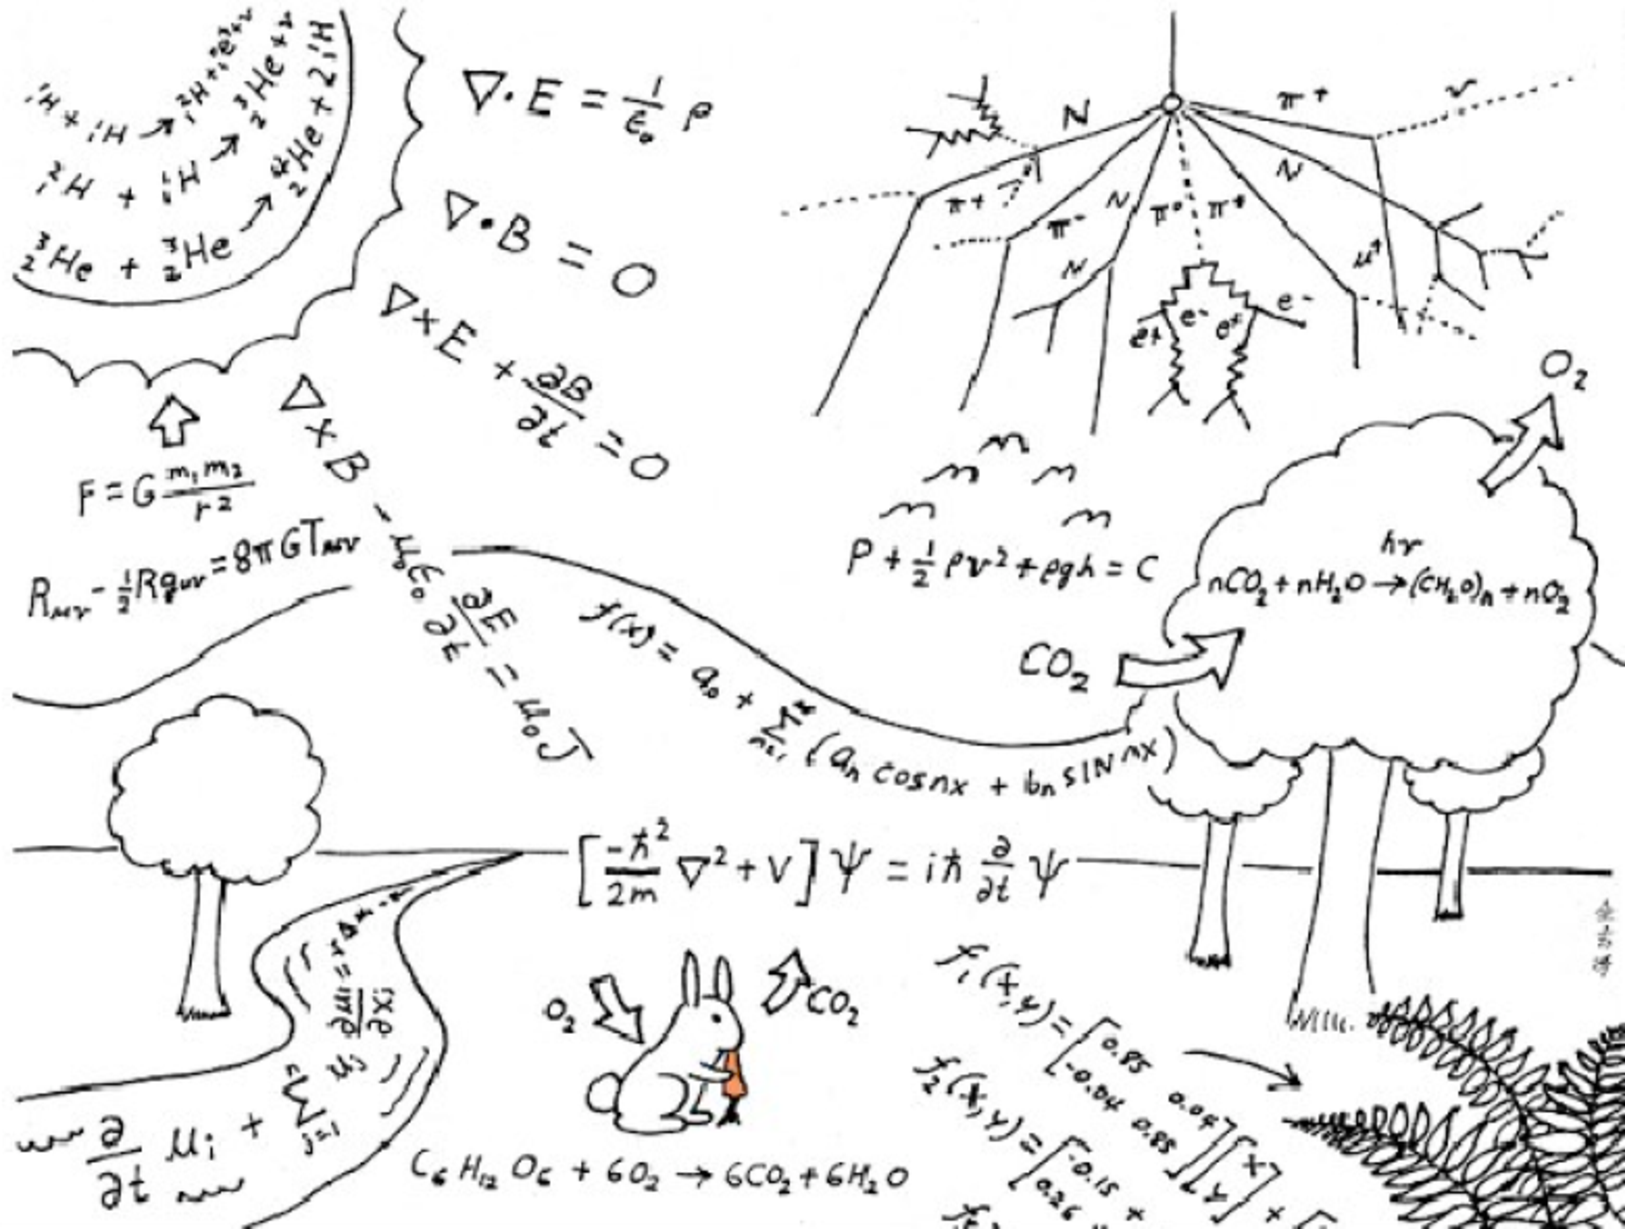
\includegraphics[width=\textwidth]{eyecandy/Wiese-Modell.pdf}
        }
        \only<2->{
          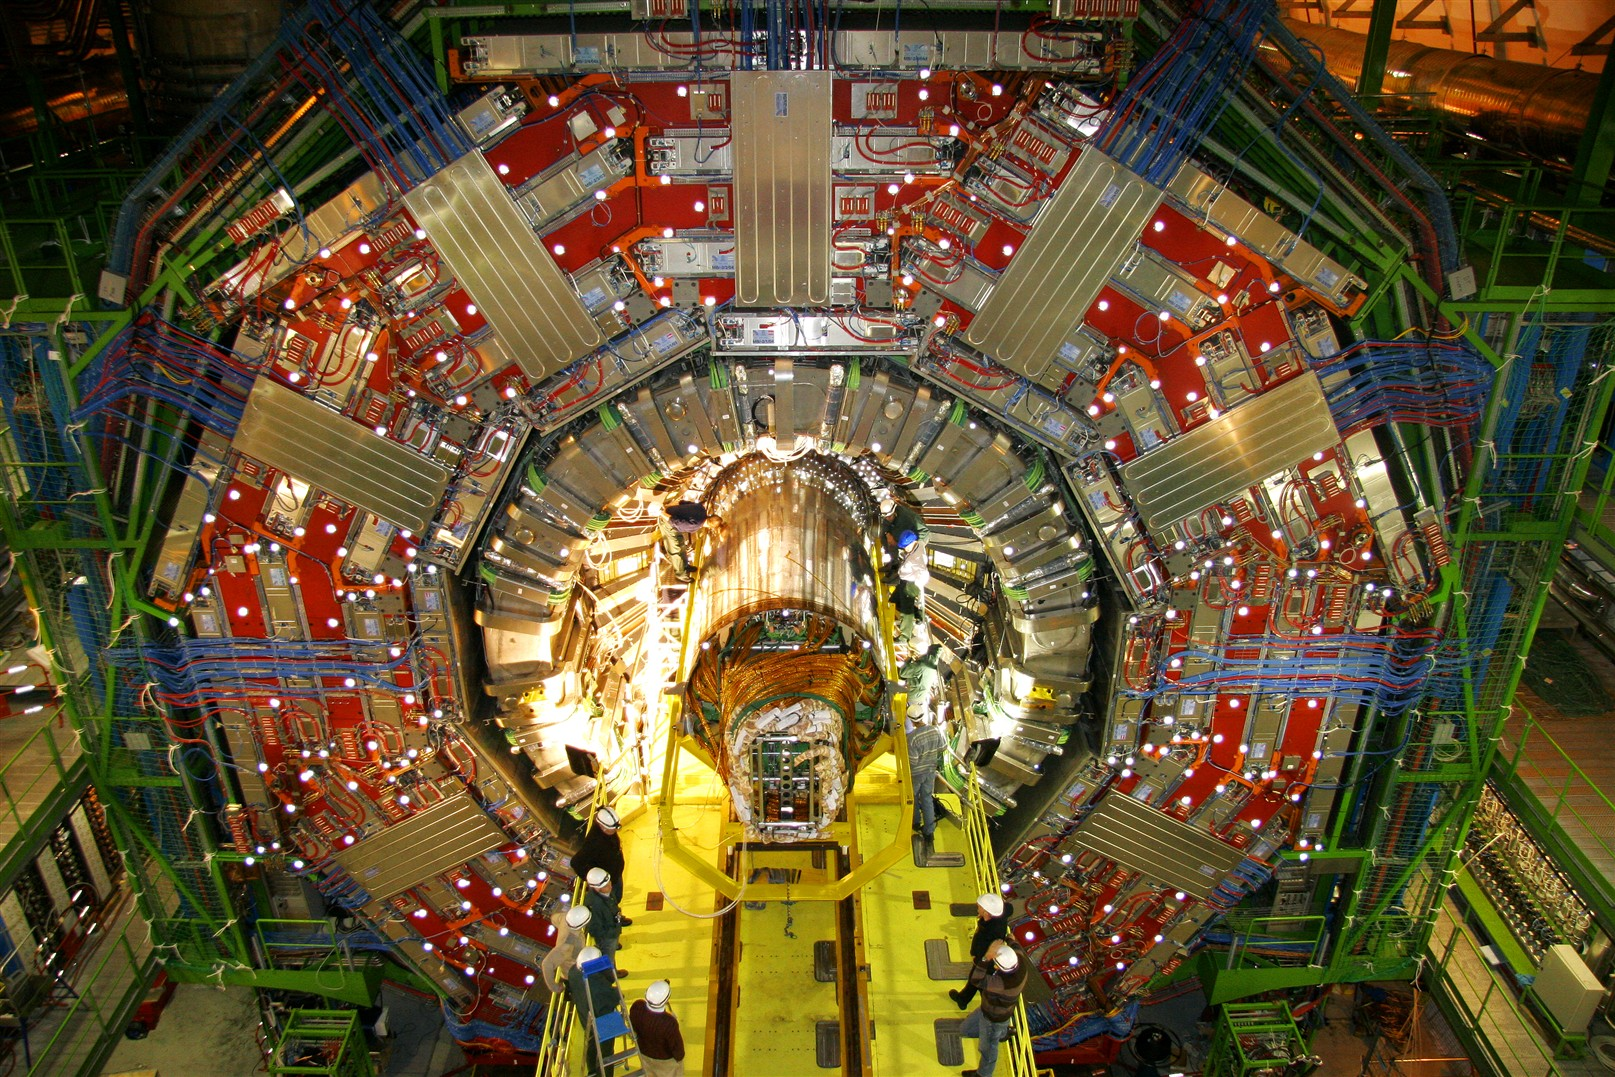
\includegraphics[width=\textwidth]{lhc/CMS_0712023_01-A4-at-144-dpi.jpg}
        }
      \end{center}
    \end{column}
    \begin{column}{0.45\textwidth}
      \visible<2->{
        \begin{center}
          \alert{Experimentalphysiker}\\
        \end{center}
        \begin{center}
          
\includegraphics[height=3cm]{eyecandy/Lennard}\\
        \end{center}
      }
      \visible<3->{
        \vskip-0.3cm
        \begin{itemize}
        \item \"Uberpr\"uft Modelle
        \item Vervollst\"andigt Modelle
          \begin{itemize}
          \item Misst z.B. Teilchenmassen
          \end{itemize}
        \item Sucht nach Unbekanntem
          \begin{itemize}
          \item z.B. Dunkle Materie
          \end{itemize}
        \end{itemize}
      }
    \end{column}
  \end{columns}
\end{frame}

% --------------------------------------------------
\begin{frame}
  \begin{center}
    {\Huge Experiment}
  \end{center}
  %\vskip0.5cm
   \begin{block}{}
     \begin{columns}
       \begin{column}{0.3\textwidth}
         \centering
         
\includegraphics[height=0.3\textheight]{eyecandy/Lennard}
       \end{column}
       \begin{column}{0.7\textwidth}
         {\large Frage:}
         \vskip0.2cm
         \alert{``Welcher geometrische K\"orper verbirgt\\ sich in dem Knetball?''}
       \end{column}
     \end{columns}
   \end{block}
\end{frame}


% ==================================================
\section{Gr\"o\ss{}enordnungen}
% --------------------------------------------------
\begin{frame}
  \frametitle{Wie gro\ss{} sind Elementarteilchen?}
  \vskip-0.2cm
  \begin{columns}[T]
    \begin{column}{0.25\textwidth}
      \centering
      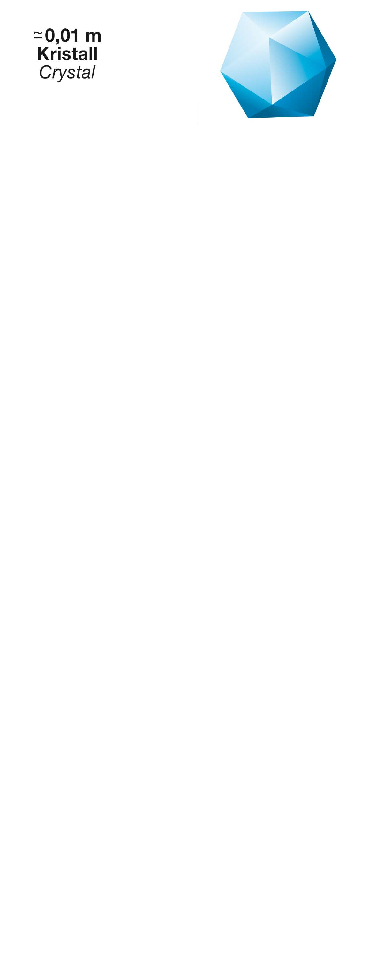
\includegraphics[width=\textwidth]{matter/VKZQ_Kristall.png}
    \end{column}
    \begin{column}{0.75\textwidth}
      \centering
      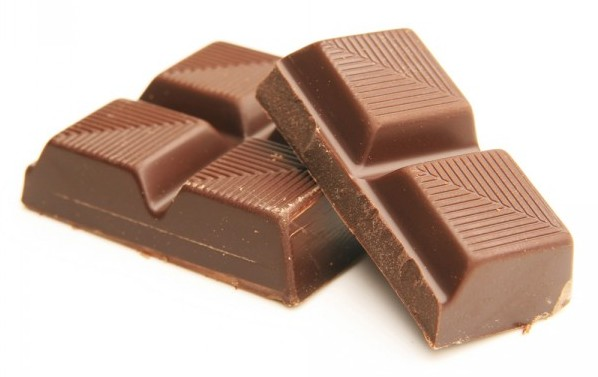
\includegraphics[width=0.7\textwidth]{matter/schokolade.jpg}\\
      \vskip0.3cm
      Materialphysik $\approx1\cm$
      \visible<2->{
        \begin{columns}
          \begin{column}{0.1\textwidth}
          \end{column}
          \begin{column}{0.2\textwidth}
            \centering
            
\includegraphics[width=\textwidth]{matter/Lupe.png}
          \end{column}
          \begin{column}{0.7\textwidth}
            \alert{Wir schauen genauer hin\ldots}
          \end{column}
        \end{columns}
      }
    \end{column}
  \end{columns}
\end{frame}

% --------------------------------------------------
\begin{frame}
  \frametitle{Wie gro\ss{} sind Elementarteilchen?}
  \vskip-0.2cm
  \begin{columns}[T]
    \begin{column}{0.25\textwidth}
      \centering
      \only<1>{
        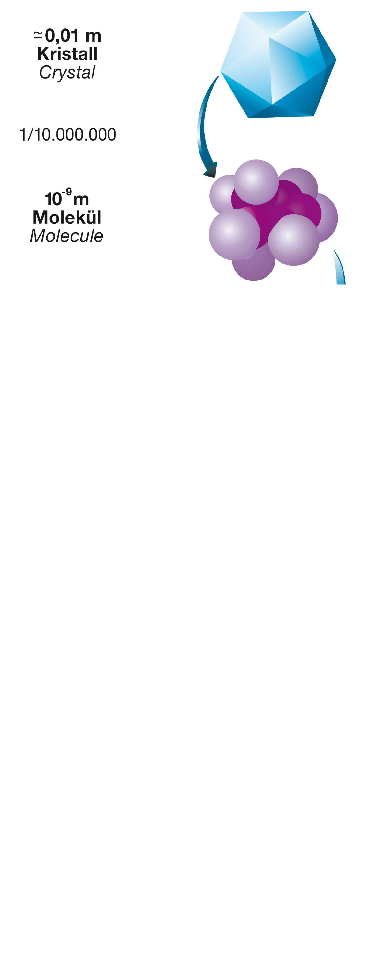
\includegraphics[width=\textwidth]{matter/VKZQ_Molekuel.png}
      }
      \only<2->{
        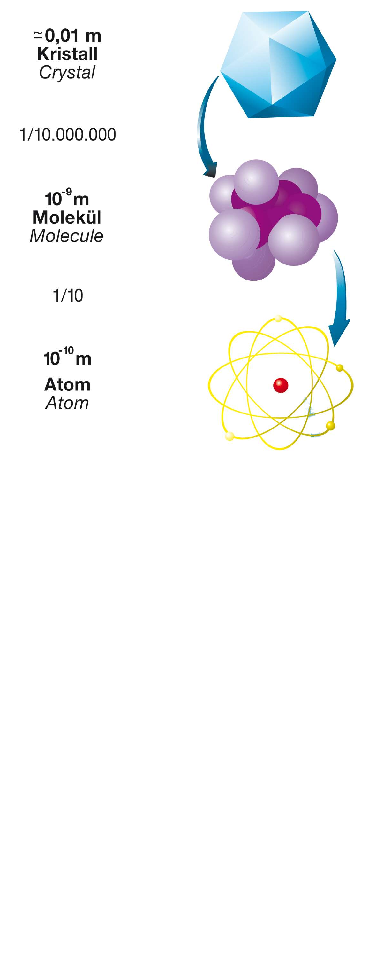
\includegraphics[width=\textwidth]{matter/VKZQ_Atom.png}
      }
    \end{column}
    \begin{column}{0.75\textwidth}
      \centering
      Molek\"ule $\approx10^{-9}\m$, Atome $\approx10^{-10}\m$
      % 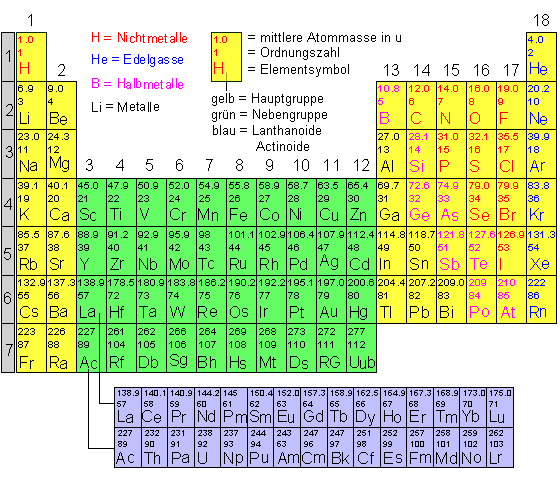
\includegraphics[width=0.7\textwidth]{matter/periodensystem.png}\\
      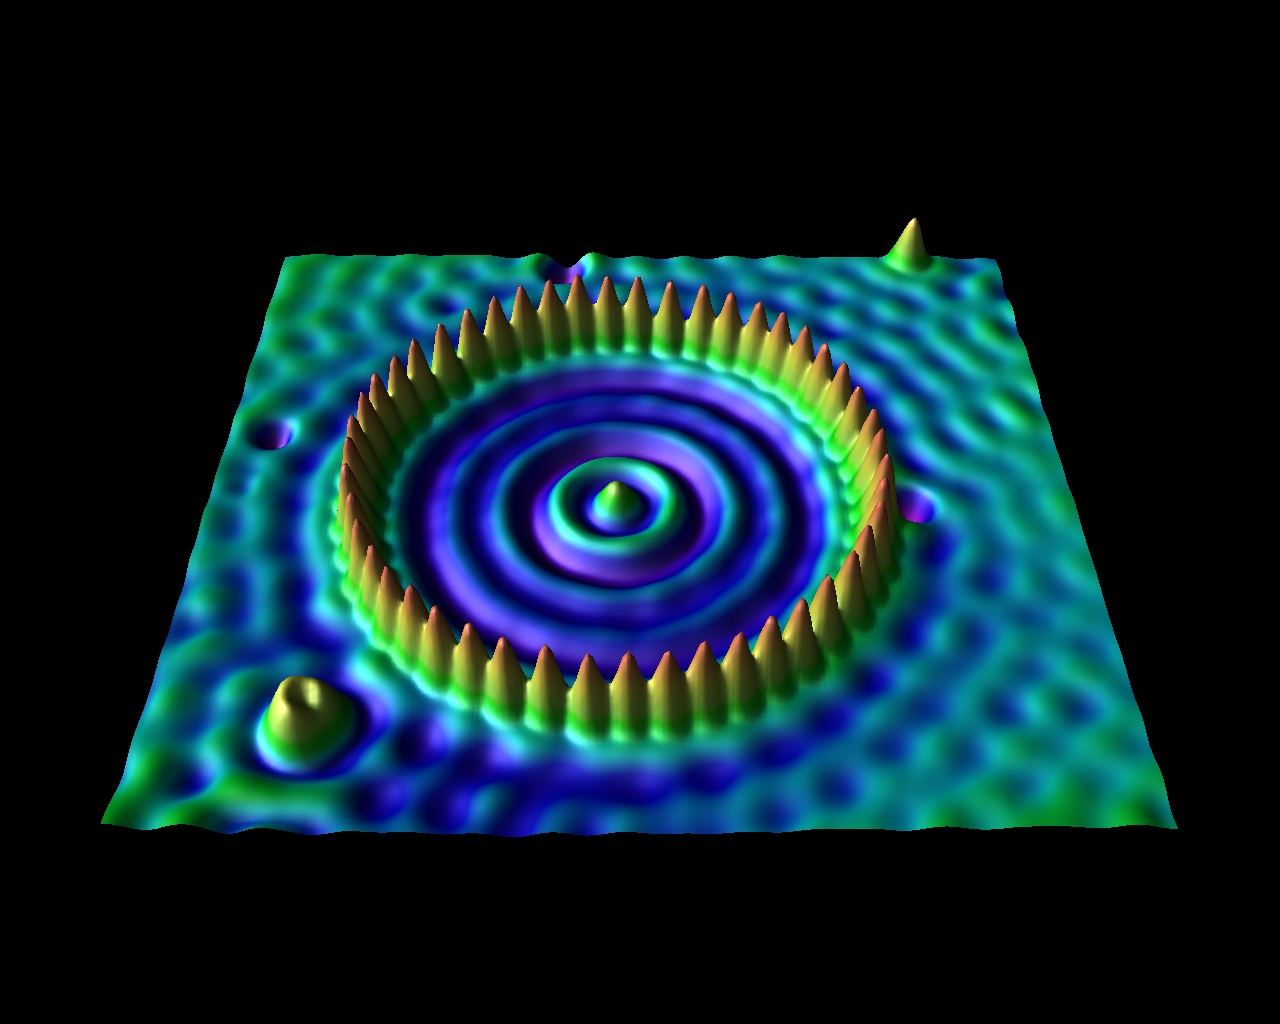
\includegraphics[width=0.7\textwidth]{matter/quantum_corral_nise.jpg}\\
      \vskip0.2cm
      \begin{block}{}
        \centering
        \alert{Atome sind Bausteine f\"ur alle makroskopischen Objekte}
      \end{block}
    \end{column}
  \end{columns}
\end{frame}

% --------------------------------------------------
\begin{frame}
  \frametitle{Wie gro\ss{} sind Elementarteilchen?}
  \vskip-0.2cm
  \begin{columns}[T]
    \begin{column}{0.25\textwidth}
      \centering
      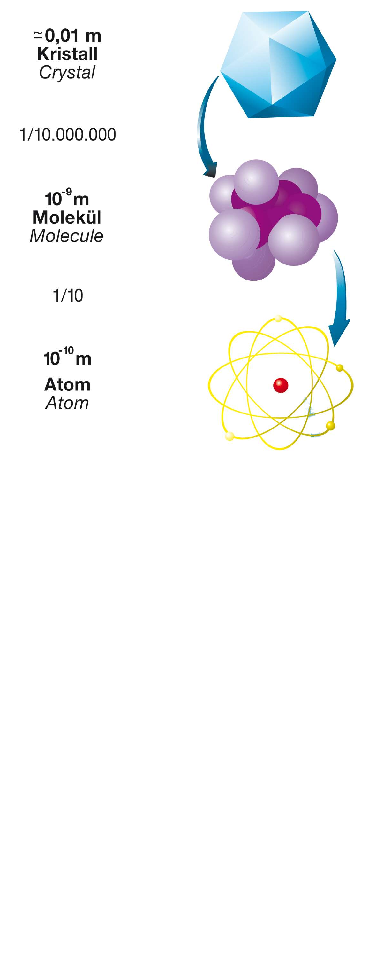
\includegraphics[width=\textwidth]{matter/VKZQ_Atom.png}
    \end{column}
    \begin{column}{0.75\textwidth}
      \centering
      \alert{Wie gro\ss{} sind $10^{-10}\m$?}
      \begin{columns}
        \begin{column}{0.1\textwidth}
        \end{column}
        \begin{column}{0.35\textwidth}
          \centering 
          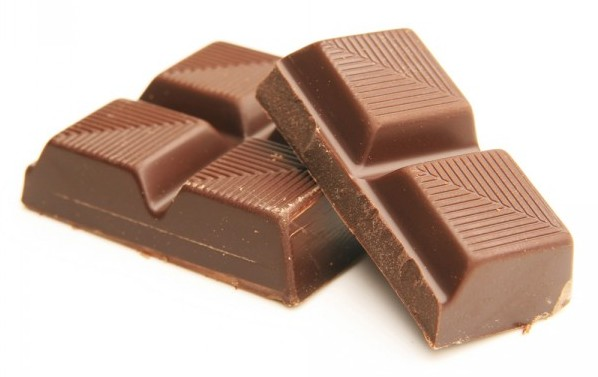
\includegraphics[height=0.18\textheight]{matter/schokolade.jpg}\\
          Schokolade
        \end{column}
        \begin{column}{0.1\textwidth}
          \centering
          {\Huge :}
        \end{column}
        \begin{column}{0.35\textwidth}
          \centering
          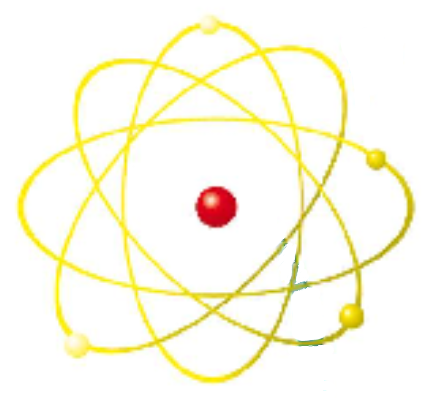
\includegraphics[height=0.18\textheight]{matter/Atom.png}\\
          Atom
        \end{column}
        \begin{column}{0.1\textwidth}
        \end{column}
      \end{columns}
      \begin{center}
        \visible<2->{\Huge =}
      \end{center}
      \begin{columns}
        \begin{column}{0.1\textwidth}
        \end{column}
        \begin{column}{0.35\textwidth}
          \centering
          \visible<2->{
            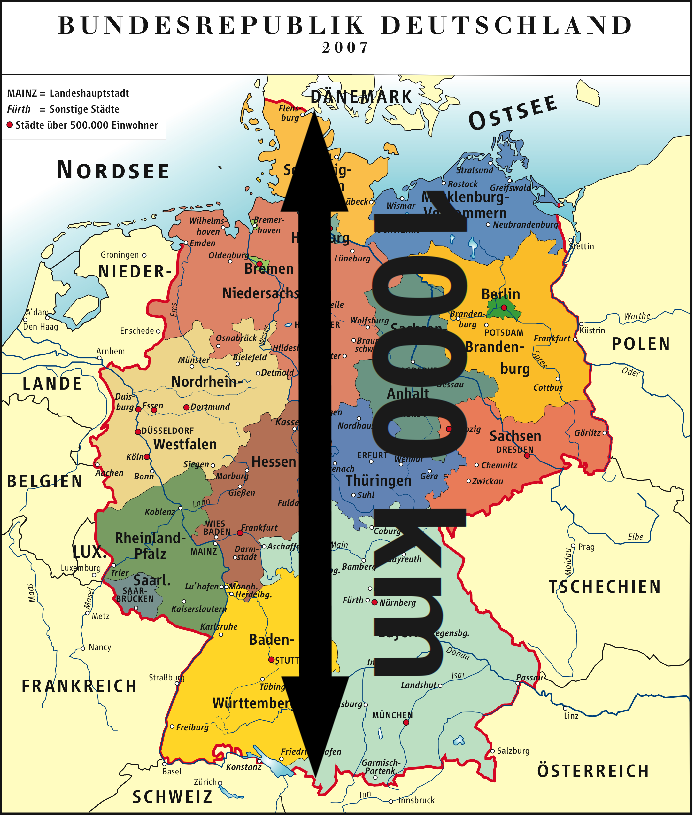
\includegraphics[width=\textwidth]{matter/DeutschlandMitMassstab.png}
          }
        \end{column}
        \begin{column}{0.1\textwidth}
          \centering
          \visible<2->{\Huge :}
        \end{column}
        \begin{column}{0.35\textwidth}
          \centering
          \only<2>{
            {\Huge ?}
          }
          \only<3->{
            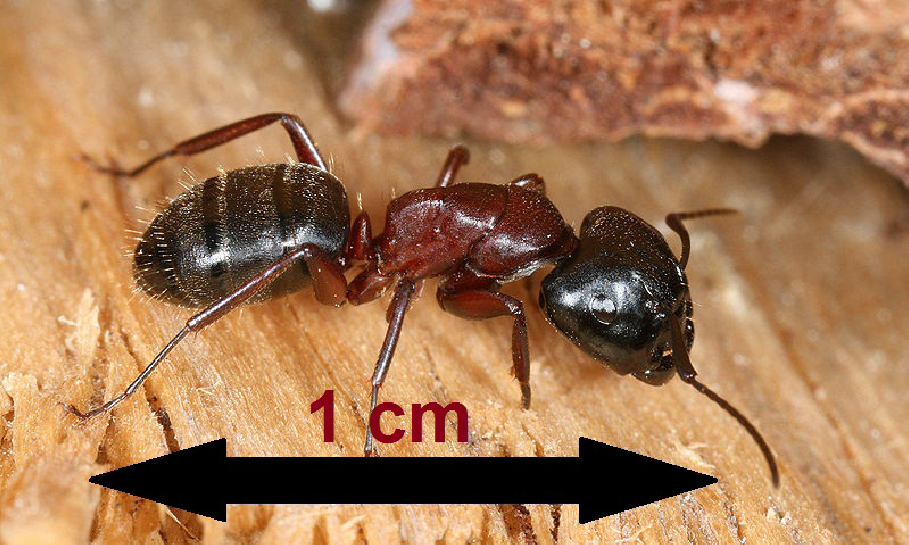
\includegraphics[width=\textwidth]{matter/AmeiseMitMassstab.png}
          }
        \end{column}
        \begin{column}{0.1\textwidth}
        \end{column}
      \end{columns}
    \end{column}
  \end{columns}
\end{frame}

% --------------------------------------------------
\begin{frame}
  \frametitle{Wie gro\ss{} sind Elementarteilchen?}
  \vskip-0.2cm
  \begin{columns}[T]
    \begin{column}{0.25\textwidth}
      \centering
      \only<1>{
        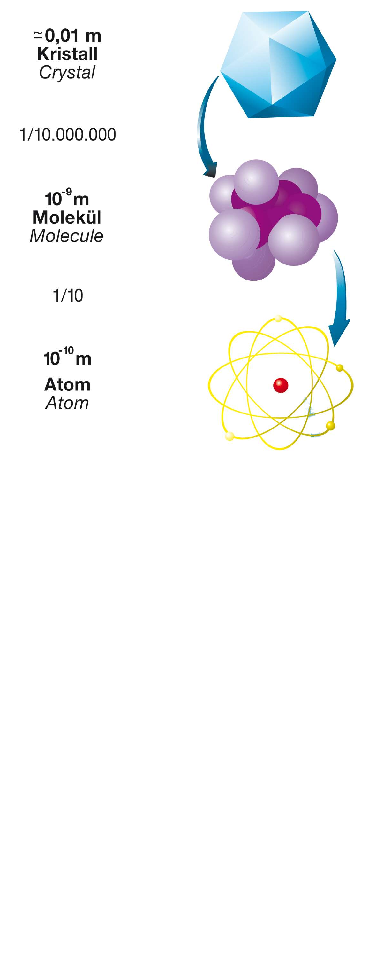
\includegraphics[width=\textwidth]{matter/VKZQ_Atom.png}
      }
      \only<2>{
        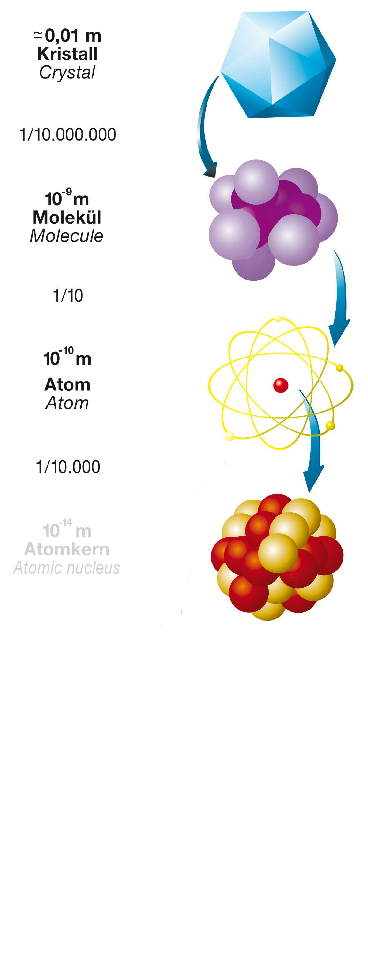
\includegraphics[width=\textwidth]{matter/VKZQ_Kern.png}
      }
      \only<3->{
        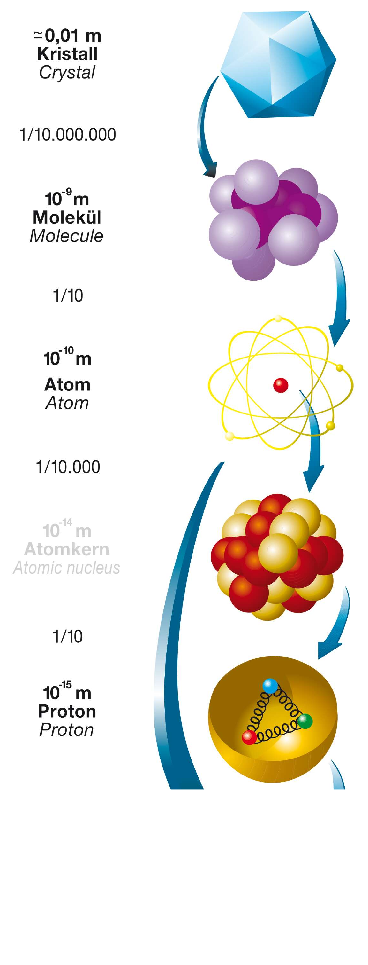
\includegraphics[width=\textwidth]{matter/VKZQ_Proton.png}
      }
    \end{column}
    \begin{column}{0.75\textwidth}
      \vskip1cm
      \begin{columns}
        \begin{column}{0.1\textwidth}
        \end{column}
        \begin{column}{0.2\textwidth}
          \centering
          
\includegraphics[width=\textwidth]{matter/Lupe.png}
        \end{column}
        \begin{column}{0.7\textwidth}
          \alert{Wir schauen genauer hin\ldots}
        \end{column}
      \end{columns}
      \vskip1cm
      \begin{columns}
        \begin{column}{0.2\textwidth}
        \end{column}
        \begin{column}{0.6\textwidth}
          \visible<3->{
            \begin{block}{}
              \centering
              Proton, Neutron $\approx10^{-15}\m$\\
              \textcolor{red}{\large Hier f\"angt Teilchenphysik an!}
            \end{block}
          }
        \end{column}
        \begin{column}{0.2\textwidth}
        \end{column}
      \end{columns}
    \end{column}
  \end{columns}
\end{frame}

% --------------------------------------------------
\begin{frame}
  \frametitle{Wie gro\ss{} sind Elementarteilchen?}
  \vskip-0.2cm
  \begin{columns}[T]
    \begin{column}{0.25\textwidth}
      \centering
      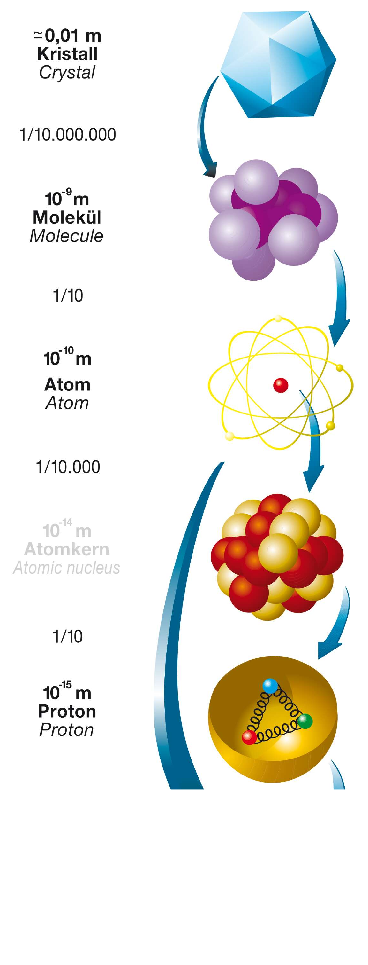
\includegraphics[width=\textwidth]{matter/VKZQ_Proton.png}
    \end{column}
    \begin{column}{0.75\textwidth}
      \centering
      \alert{Wie gro\ss{} sind $10^{-15}\m$?}
      \begin{columns}
        \begin{column}{0.1\textwidth}
        \end{column}
        \begin{column}{0.35\textwidth}
          \centering
          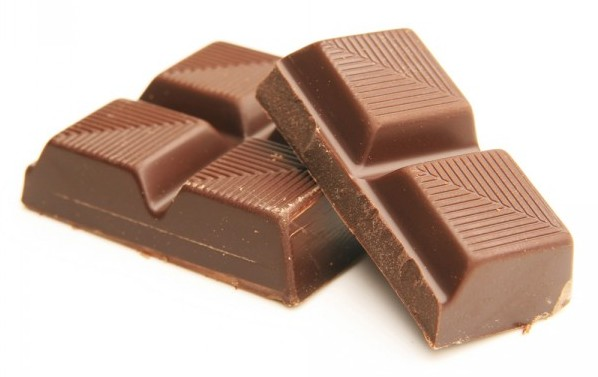
\includegraphics[height=0.18\textheight]{matter/schokolade.jpg}\\
          Schokolade
        \end{column}
        \begin{column}{0.1\textwidth}
          \centering
          {\Huge :}
        \end{column}
        \begin{column}{0.35\textwidth}
          \centering
          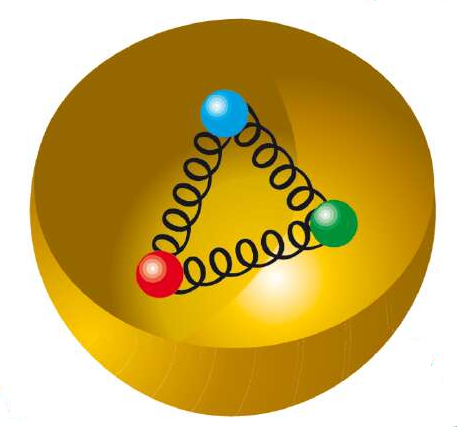
\includegraphics[height=0.18\textheight]{matter/Proton.png}\\
          Proton
        \end{column}
        \begin{column}{0.1\textwidth}
        \end{column}
      \end{columns}
      \begin{center}
        \visible<2->{\Huge =}
      \end{center}
      \begin{columns}
        \begin{column}{0.1\textwidth}
        \end{column}
        \begin{column}{0.35\textwidth}
          \centering
          \only<2>{
            {\Huge ?}
          }
          \only<3->{
            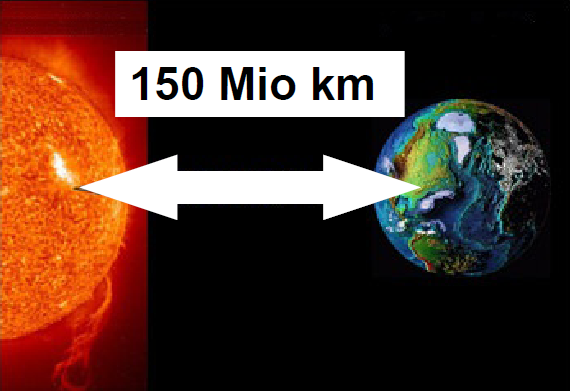
\includegraphics[width=\textwidth]{matter/ErdeSonne.png}
          }
        \end{column}
        \begin{column}{0.1\textwidth}
          \centering
          \visible<2->{\Huge :}
        \end{column}
        \begin{column}{0.35\textwidth}
          \centering
          \visible<2->{
            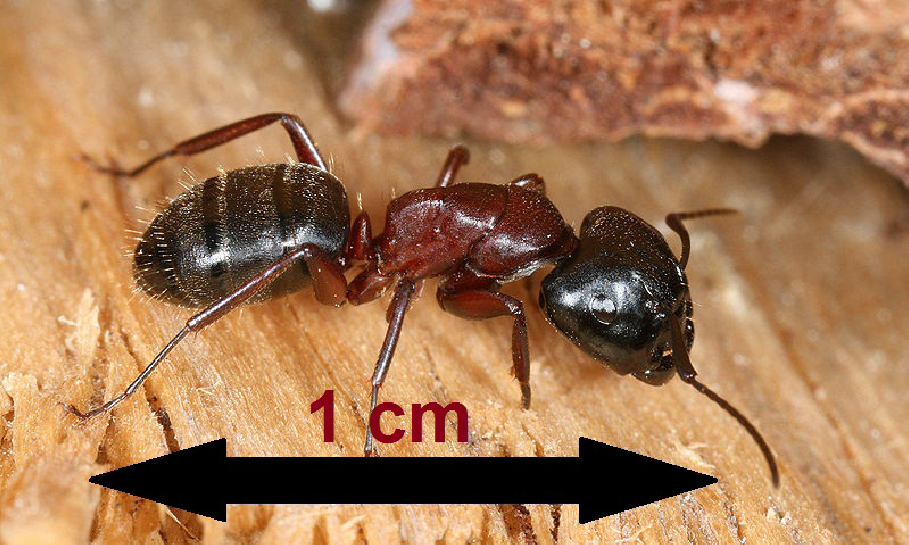
\includegraphics[width=\textwidth]{matter/AmeiseMitMassstab.png}
          }
        \end{column}
        \begin{column}{0.1\textwidth}
        \end{column}
      \end{columns}
    \end{column}
  \end{columns}
\end{frame}

% --------------------------------------------------
\begin{frame}
  \frametitle{Wie gro\ss{} sind Elementarteilchen?}
  \vskip-0.2cm
  \begin{columns}[T]
    \begin{column}{0.25\textwidth}
      \centering
      \only<1>{
        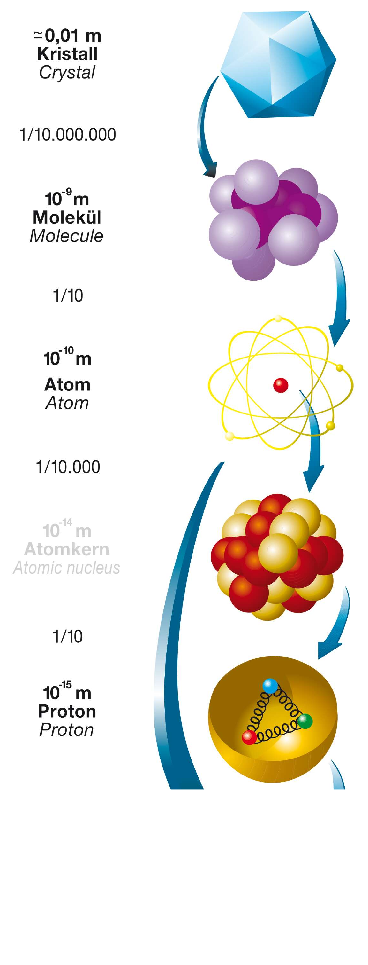
\includegraphics[width=\textwidth]{matter/VKZQ_Proton.png}
      }
      \only<2->{
        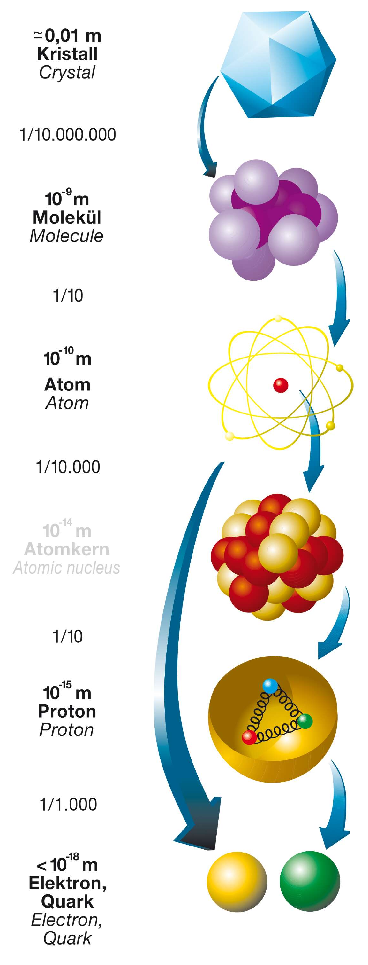
\includegraphics[width=\textwidth]{matter/VKZQ_Alles.png}
      }
    \end{column}
    \begin{column}{0.75\textwidth}
      \vskip1cm
      \begin{columns}
        \begin{column}{0.1\textwidth}
        \end{column}
        \begin{column}{0.2\textwidth}
          \centering
          
\includegraphics[width=\textwidth]{matter/Lupe.png}
        \end{column}
        \begin{column}{0.7\textwidth}
          \alert{Wir schauen genauer hin\ldots}
        \end{column}
      \end{columns}
      \vskip0.5cm
      \begin{columns}
        \begin{column}{0.1\textwidth}
        \end{column}
        \begin{column}{0.8\textwidth}
          \visible<2->{
            \begin{block}{}
              \centering
              Quarks, Elektronen
              \vskip0.3cm
              \textcolor{red}{\Huge Elementarteilchen}
            \end{block}
            \begin{itemize}
            \item $<10^{-18}\m$ \visible<3->{(experimentell)}
            \item<3-> punktf\"ormig (theoretisch)
            \end{itemize}
          }
        \end{column}
        \begin{column}{0.1\textwidth}
        \end{column}
      \end{columns}
    \end{column}
  \end{columns}
\end{frame}


% ==================================================
\section{Das Standardmodell}
\subsection{Elementarteilchen}
% --------------------------------------------------
\begin{frame}[t]
  \frametitle{Sichtbare Materie}
  \begin{itemize}
  \item Woraus besteht die sichtbare Welt?
  \item Woraus bestehen wir?
  \end{itemize}
  \vskip0.3cm
  \begin{columns}
    \begin{column}{0.25\textwidth}
      \vskip1.5cm
      \centering
      \visible<4->{
        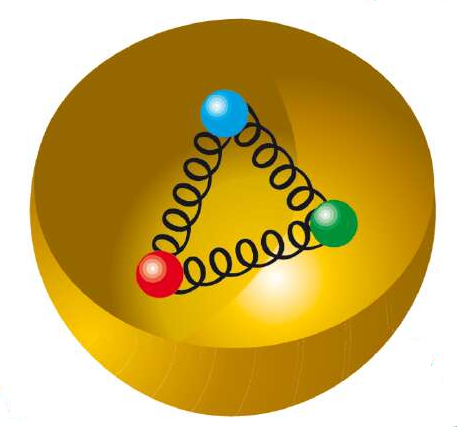
\includegraphics[width=0.8\textwidth]{matter/Proton.png}
      }
    \end{column}
    \begin{column}{0.55\textwidth}
      \only<1-6>{{\huge Atome}}
      \only<7>{\textcolor{red}{\huge Elementarteilchen}}
      \vskip0.1cm
      \begin{itemize}
      \item<2-> Atomh\"ulle
        \begin{itemize}
        \item<3-> \textcolor{red}{Elektronen}: $Q=-1$
        \end{itemize}
      \item<2-> Atomkern
        \begin{itemize}
        \item<4-> Protonen: $Q=+1$
          \visible<5->{
            \begin{center}
              \begin{tabular}{ll}
                2 \textcolor{red}{up quarks} & $Q=+2/3$  \\
                1 \textcolor{red}{down quark}& $Q=-1/3$ \\
              \end{tabular}
            \end{center}
          }
        \item<4-> Neutronen: $Q=0$
          \visible<6->{
            \begin{center}
              \begin{tabular}{ll}
                1 \textcolor{red}{up quark} & $Q=+2/3$  \\
                2 \textcolor{red}{down quarks}& $Q=-1/3$ \\
              \end{tabular}
            \end{center}
          }
        \end{itemize}
      \end{itemize}
    \end{column}
    \begin{column}{0.2\textwidth}
      \centering
      \vskip-3cm
      \hskip-2cm
      \visible<2->{
        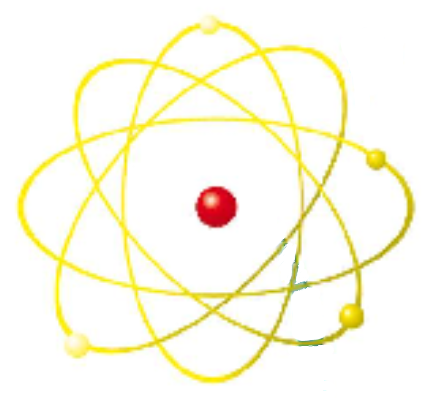
\includegraphics[width=\textwidth]{matter/Atom.png}
      }
    \end{column}
  \end{columns}
\end{frame}

% --------------------------------------------------
\begin{frame}[t]
  \frametitle{Sichtbare Materie}
  \begin{itemize}
  \item Woraus besteht die sichtbare Welt?
  \item Woraus bestehen wir?
  \end{itemize}
  \vskip0.3cm
  \begin{columns}
    \begin{column}{0.25\textwidth}
      \centering
      \vskip0.5cm
      \visible<3->{
        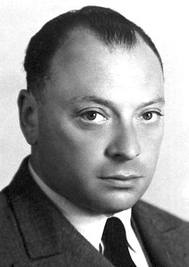
\includegraphics[width=0.8\textwidth]{sm/Pauli.jpg}\\
        W.\ Pauli        
      }
    \end{column}
    \begin{column}{0.55\textwidth}
      \only<1->{\textcolor{white}{\huge Elementarteilchen}}
      \vskip0.1cm
      \visible<2->{
        Neutron ist instabil: $\beta$-Zerfall
        \begin{equation*}
          n \rightarrow p + e^{-} \visible<3->{+\textcolor{red}{\bar{\nu}_{e}}}
        \end{equation*}
        \only<2>{{\Large Problem:} keine Energieerhaltung!}
        \only<3->{1932: \textcolor{red}{\Large Neutrino}}
      }
    \end{column}
    \begin{column}{0.2\textwidth}
    \end{column}
  \end{columns}
\end{frame}

% --------------------------------------------------
\begin{frame}[t]
  \frametitle{Sichtbare Materie}
  \begin{itemize}
  \item Woraus besteht die sichtbare Welt?
  \item Woraus bestehen wir?
  \end{itemize}
  \vskip0.3cm
  \begin{columns}
    \begin{column}{0.25\textwidth}
      \centering
      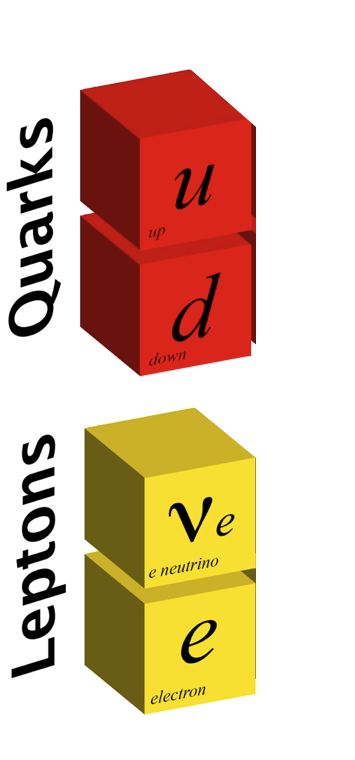
\includegraphics[width=\textwidth]{sm/StandardModel_FirstGeneration.png}
    \end{column}
    \begin{column}{0.75\textwidth}
      \textcolor{red}{\huge 4 Elementarteilchen}
      \visible<2->{
        \begin{center}
          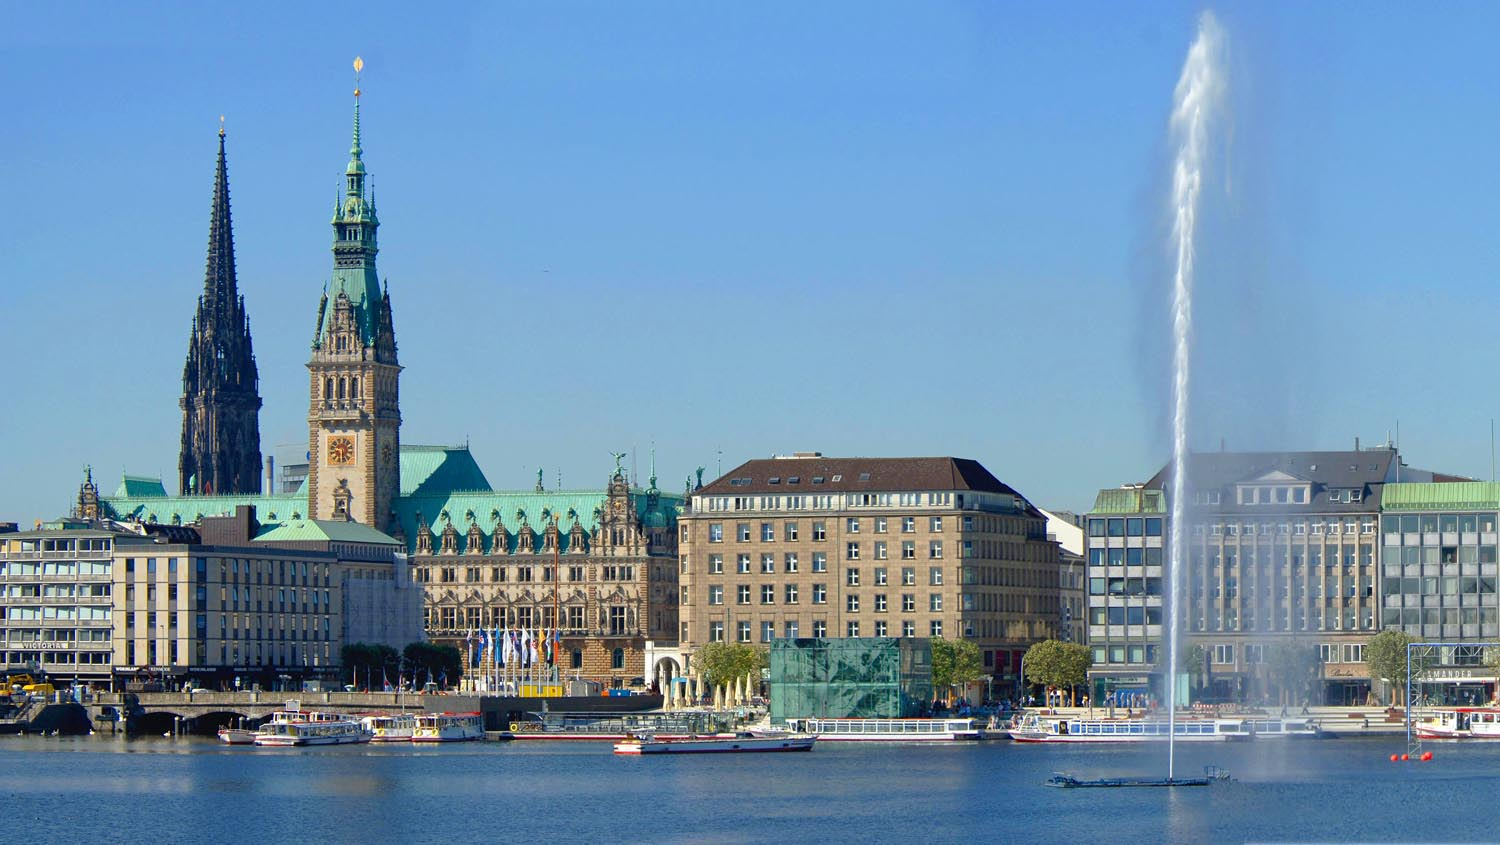
\includegraphics[height=0.25\textheight]{matter/Hamburg_Jungfernstieg.jpg}
          \hskip0.5cm
          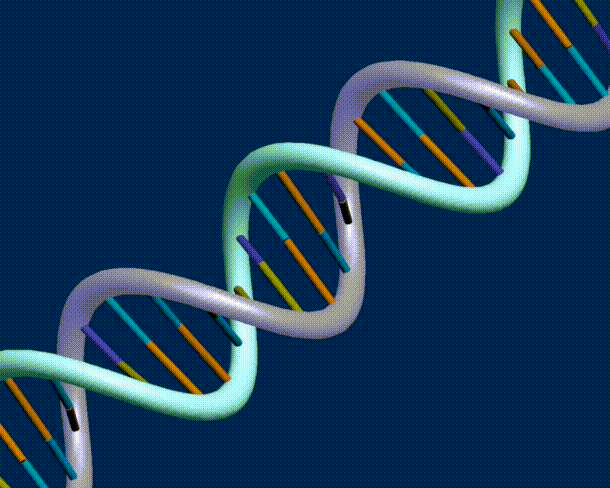
\includegraphics[height=0.2\textheight]{matter/DNA.png}\\
          \vskip0.2cm
          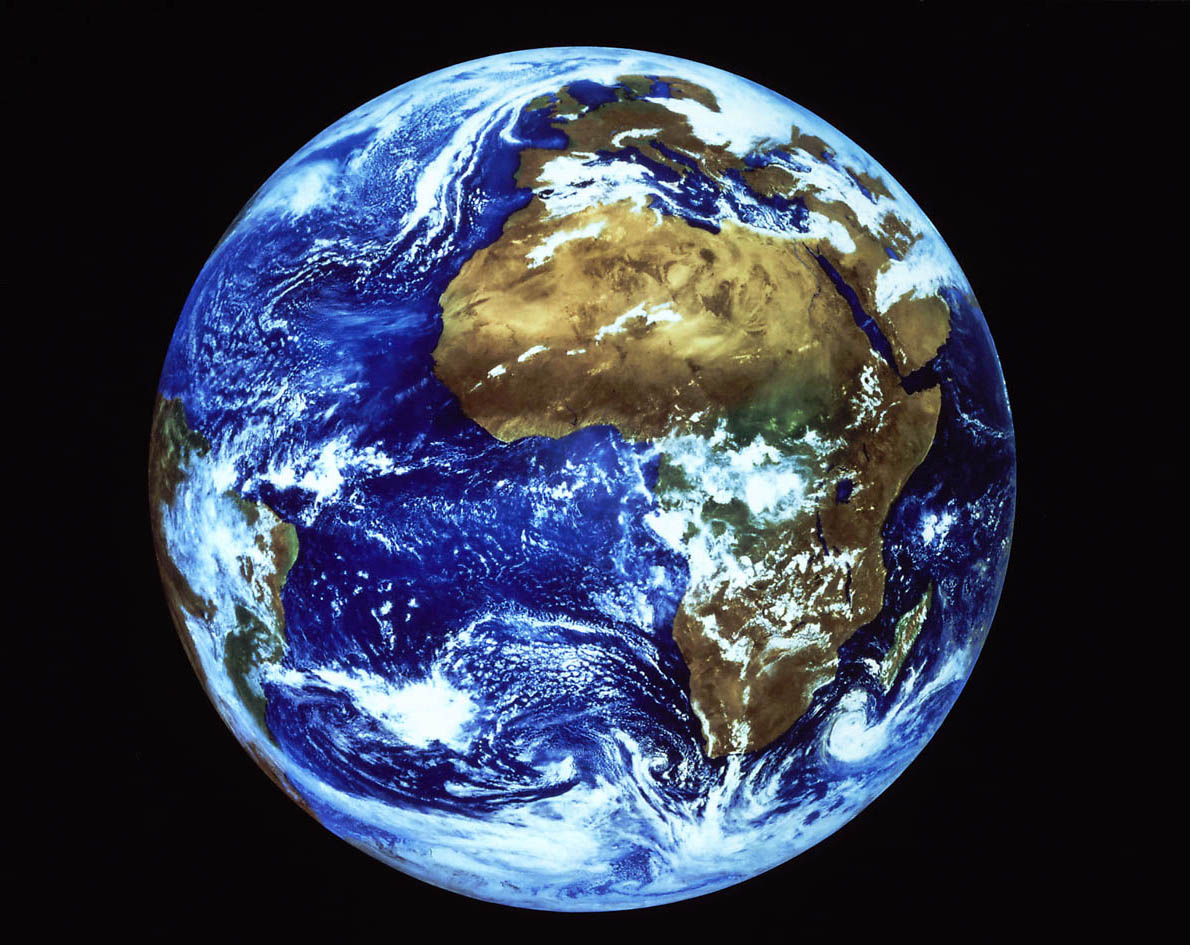
\includegraphics[height=0.23\textheight]{matter/earth.jpg}
          \hskip0.8cm
          \includegraphics[height=0.2\textheight]{matter/Volldampf.jpg}
          \hskip0.8cm
          \includegraphics[height=0.21\textheight]{matter/Katy-Perry.jpg}
        \end{center}
        \begin{flushright}
          \vskip-0.3cm
          \textcolor{red}{\large zur Beschreibung der sichtbaren Materie!}
        \end{flushright}
      }
    \end{column}
  \end{columns}
\end{frame}

\subsection{Weitere Generationen}
% --------------------------------------------------
\begin{frame}
  \frametitle{Gibt es noch weitere Elementarteilchen?}
  \begin{columns}
    \begin{column}{0.6\textwidth}
      \begin{itemize}
      \item 1936: Ein neues Elementarteilchen
        \begin{itemize}
        \item In kosmischer H\"ohenstrahlung
        \end{itemize}
      \item Das Myon $\mu^{-}$
        \begin{itemize}
        \item Gleiche elektrische Ladung wie $e^{-}$
        \item 200 mal schwerer als $e^{-}$
        \item Instabil ($\mu^{-}\rightarrow e^{-} + \bar{\nu}_{e} + \nu_{\mu}$)
        \end{itemize}
      \end{itemize}
      \visible<2->{
        \begin{columns}
          \begin{column}{0.1\textwidth}
          \end{column}
          \begin{column}{0.4\textwidth}
            \centering
            \includegraphics[width=\textwidth]{sm/StandardModel_FirstGenerationPlusMuon.png}
          \end{column}
          \begin{column}{0.5\textwidth}
            \begin{center}
              \textcolor{red}{\Large Myon $\mu^{-}$}\\
              ``Schweres Elektron''
            \end{center}
          \end{column}
        \end{columns}
      }
    \end{column}
    \begin{column}{0.4\textwidth}
      \centering
      \includegraphics[width=\textwidth]{sm/KosmischeStrahlung.jpg}
    \end{column}
  \end{columns}
\end{frame}

% --------------------------------------------------
\begin{frame}
  \frametitle{Gibt es noch weitere Elementarteilchen?}
  \begin{columns}
    \begin{column}{0.65\textwidth}
      {\Large Sind das jetzt alle? Nein!}
      \vskip0.3cm
      Es gibt noch mehr Elemtarteilchen
      \begin{itemize}
      \item Meist \textbf{instabil} und sehr kurzlebig
        \begin{itemize}
        \item Nicht in sichtbarer Materie ``verbaut''
        \end{itemize}
      \item Oder nahezu \textbf{``unsichtbar''}
        \begin{itemize}
        \item Neutrinos
        \end{itemize}
      \end{itemize}
      \vskip0.5cm
      \begin{block}{}
        \centering
        \alert{\Large Erzeugung in Teilchenkollisionen\\ \zb am LHC}
      \end{block}
    \end{column}
    \begin{column}{0.35\textwidth}
      \centering
      \includegraphics[width=7cm,angle=90]{sm/CMS_Collision_gen-2007-004_02.jpg}
    \end{column}
  \end{columns}
\end{frame}

% --------------------------------------------------
\begin{frame}
  \begin{center}
    {\Huge Experiment Teilchenzoo}
  \end{center}
  %\vskip0.5cm
   \begin{block}{}
     \begin{columns}
       \begin{column}{0.3\textwidth}
         \centering
         \includegraphics[height=0.3\textheight]{eyecandy/Lennard}
       \end{column}
       \begin{column}{0.7\textwidth}
         \alert{``Ordne die Elementarteilchen anhand\\ ihrer Eigenschaften.''}
       \end{column}
     \end{columns}
   \end{block}
\end{frame}

\subsection{Die bekannten Elementarteilchen}
% --------------------------------------------------
\begin{frame}
  \frametitle{Die bekannten Elementarteilchen}
  \vskip-0.8cm
  \begin{columns}[T]
    \begin{column}{0.5\textwidth}
      \begin{center}
        \only<1-4>{
          \includegraphics[width=0.95\textwidth]{sm/SM-Table.png}\\
        }
        \only<5->{
          \includegraphics[width=0.95\textwidth]{sm/SM-Table_Antimatter.png}\\
        }
      \end{center}
      \vskip-3cm
      \visible<3>{
        \includegraphics[width=0.5\textwidth]{sm/VWKaefer.jpg}\\
      }
    \end{column}
    \begin{column}{0.5\textwidth}
      \begin{block}{Ordnung}
        \begin{itemize}
        \item Masse
        \item Quantenzahlen
          \begin{itemize}
          \item Z.B.\ Ladung
          \end{itemize}
        \end{itemize}
      \end{block}
      \visible<2->{
        \begin{block}{Teilchen der 2. und 3. Generation}
          \begin{itemize}
          \item Gleiche Eigenschaften wie 1.
          \item Aber deutlich schwerer
            \begin{itemize}
            \item Instabil
            \end{itemize}
          \end{itemize}
        \end{block}
      }
      \visible<5->{
        \begin{block}{Zu jedem Teilchen: Antiteilchen}
          \begin{itemize}
          \item Gleiche Eigenschaften
          \item Aber entgegengesetzte Ladung
            \begin{itemize}
            \item Z.B.\ $e^{-}$ und $e^{+}$
            \end{itemize}
          \end{itemize}
        \end{block}
      }
      \vskip-7cm
      \visible<3>{
        \includegraphics[width=0.5\textwidth]{sm/QueenMary2.jpg}\\
      }
    \end{column}
  \end{columns}
\end{frame}


\subsection{Fundamentale Kr\"afte}
% --------------------------------------------------
\begin{frame}[t]
  \frametitle{Kr\"afte: Interaktion zwischen den Elementarteilchen}
  \begin{block}{}
    \begin{itemize}
    \item Kr\"afte wirken zwischen \textcolor{red}{geladenen Teilchen}
    \item Kr\"afte entstehen durch den \textcolor{green}{Austausch von
        Teilchen (``Bosonen'')}
    \end{itemize}
  \end{block}
  \begin{center}
    \includegraphics[width=0.95\textwidth]{sm/interact.jpg}
  \end{center}
  \only<2>{
    \begin{itemize}
    \item Anschauliche (und mathematische!) Beschreibung durch ``Feynmandiagramme''
    \end{itemize}
  }
  \only<3->{
    \begin{itemize}
    \item Z.B.\ \textcolor{red}{Elektron-Elektron Absto\ss{}ung} durch \textcolor{green}{Photon-Austausch}
    \item Elektromagnetische Kraft
    \end{itemize}
  }
\end{frame}

% --------------------------------------------------
\begin{frame}
  \frametitle{Fundamentale Kr\"afte}
  \vskip-0.2cm
  \begin{block}{Elektromagnetische Kraft}
   \begin{columns}[T]
     \begin{column}{0.7\textwidth}
        \begin{itemize}
        \item Elektrische Ladung, alle au\ss{}er $\nu$
        \item Vermittelt durch Photon $\gamma$
        \item \textit{Chemie, Elektrizit\"at}
        \end{itemize}
      \end{column}
      \begin{column}{0.3\textwidth}
        \centering
        \vskip-0.3cm
        \includegraphics[height=0.22\textheight]{matter/Atom.png}
      \end{column}
    \end{columns}
  \end{block}
  \pause
  \begin{block}{Schwache Kraft}
    \begin{columns}[T]
      \begin{column}{0.7\textwidth}
        \begin{itemize}
        \item Schwache Ladung, alle Teilchen
        \item Vermittelt durch $W^{\pm}$, \textcolor{red}{$\znull$}
        \item \textit{Umwandlung von Teilchensorten ($\beta$-, $\mu$-Zerfall)}
        \end{itemize}
      \end{column}
      \begin{column}{0.3\textwidth}
        \centering
        \vskip-0.3cm
        \includegraphics[height=0.22\textheight]{sm/BetaZerfall.pdf}
      \end{column}
    \end{columns}
  \end{block}
  \pause
  \begin{block}{Starke Kraft}
    \begin{columns}[T]
      \begin{column}{0.7\textwidth}
        \begin{itemize}
        \item Farbladung (drei Zust\"ande \textcolor{red}{r}\textcolor{green}{g}\textcolor{blue}{b}), nur Quarks
        \item Vermittelt durch Gluon $g$
        \item \textit{Bindung der Quarks in Hadronen: $qqq$, $q\bar{q}$}
       \end{itemize}
      \end{column}
      \begin{column}{0.3\textwidth}
        \centering
        \vskip-0.3cm
        \includegraphics[height=0.22\textheight]{matter/Proton.png}
      \end{column}
    \end{columns}
  \end{block}
\end{frame}

\subsection{Zusammenfassung}
% --------------------------------------------------
\begin{frame}
  \frametitle{Das Standardmodell der Teilchenphysik}
  \begin{columns}
    \begin{column}{0.5\textwidth}
      \begin{center}
        \includegraphics[width=0.9\textwidth]{sm/sm_blocks_wo_higgs.jpg}
      \end{center}
    \end{column}
    \begin{column}{0.5\textwidth}
      \begin{itemize}
      \item Einheitliche Beschreibung der
        \begin{itemize}
        \item fundamentalen Teilchen und ihrer Eigenschaften
        \item fundamentalen Kr\"afte (ausgenommen
          Gravitation)
        \end{itemize}
      \item Beruht auf
        \begin{itemize}
        \item Spezieller Relativit\"atstheorie
        \item Quantenmechanik
        \end{itemize}
      \item Genaueste Beschreibung der Natur
      \end{itemize}
   \end{column}
  \end{columns}
  \pause
  \vskip0.5cm
  \begin{block}{}
    \begin{center}
      \textit{``Das Standardmodell funktioniert frustrierend gut.''}
      {\scriptsize R.~Heuer, 2011}
    \end{center}
  \end{block}
\end{frame}


% ==================================================
\section{Offene Fragen}
% --------------------------------------------------
\begin{frame}
  \frametitle{Woher bekommen die Teilchen Masse?}
  \begin{columns}
    \begin{column}{0.6\textwidth}
      \begin{itemize}
      \item Standardmodell erlaubt keine Massen
      \item \alert{Elementarteilchen haben Massen!}
      \end{itemize}
    \end{column}
    \begin{column}{0.4\textwidth}
      \begin{center}
        \includegraphics[width=0.4\textwidth]{sm/QueenMary2.jpg}
        \includegraphics[width=0.5\textwidth]{sm/VWKaefer.jpg}\\
        $m_{t} \approx340\,000 \cdot m_{e}$
      \end{center}
    \end{column}
  \end{columns}
  \pause
  \vskip0.5cm
  \begin{columns}
   \begin{column}{0.5\textwidth}
      \begin{block}{Higgs-Mechanismus}
        \begin{itemize}
        \item Hintergrundfeld im Universum
        \item Teilchen werden ``abgebremst''
        \item[$\Rightarrow$] \alert{Masse}
        \end{itemize}
      \end{block}
      \vskip0.2cm
      \large Vorhersage: \textcolor{red}{Higgs Teilchen}
    \end{column}
    \begin{column}{0.5\textwidth}
      \centering
      \includegraphics[width=0.9\textwidth]{sm/higgs_swim.jpg}
    \end{column}
  \end{columns}
\end{frame}

% --------------------------------------------------
\begin{frame}
  \frametitle{Die Higgs-Story}
  \vskip-0.2cm
  \begin{columns}[T]
    \begin{column}{0.2\textwidth}
      \centering
      \includegraphics[width=0.8\textwidth]{sm/PeterHiggs.jpg}
    \end{column}
    \begin{column}{0.5\textwidth}
      \begin{itemize}
      \item \"Uber 40 Jahre
      \item<2-> Viele Beschleunigerexperimente
      \item<3-> Ungez\"ahlte Teilchenphysiker
      \end{itemize}
    \end{column}
    \begin{column}{0.3\textwidth}
      \centering
      \visible<2->{
        \includegraphics[width=0.9\textwidth]{lhc/lhc_air.jpg}
      }
    \end{column}
  \end{columns}
  \vskip-0.8cm
  \begin{columns}
    \begin{column}{0.4\textwidth}
      \centering
      \visible<4->{
        \includegraphics[width=0.9\textwidth]{sm/HiggsGammaGamma.png}\\
      }
    \end{column}
    \begin{column}{0.3\textwidth}
      \begin{flushright}
        \visible<3->{
          \includegraphics[width=0.8\textwidth]{lhc/cern_first_physics_lhc_10-620x.jpg}
        }
      \end{flushright}
      \centering
      \visible<4->{
        \includegraphics[width=0.9\textwidth]{lhc/HiggsJoe.jpg}
      }
    \end{column}
    \begin{column}{0.3\textwidth}
      \vskip0.3cm
      \centering
      \visible<4->{
        \includegraphics[width=0.9\textwidth]{sm/HiggsMGammaGamma.png}\\
        4. July 2012
      }
    \end{column}
  \end{columns}
  \visible<4->{
    \begin{block}{}
      \centering
      \alert{\Large Eindeutige Hinweise auf ein Higgs-artiges Teilchen!}
    \end{block}
  }
\end{frame}

% --------------------------------------------------
\begin{frame}[t]
  \vskip0.4cm
  \begin{columns}
   \begin{column}{0.2\textwidth}
     \centering
      \includegraphics[height=1.5cm]{eyecandy/Sheldon}
    \end{column}
    \begin{column}{0.6\textwidth}
      \alert{\Large Offene Fragen der Teilchenphysik}
    \end{column}
    \begin{column}{0.2\textwidth}
    \end{column}
  \end{columns}
  \vskip0.5cm
  \begin{columns}
    \begin{column}{0.7\textwidth}
      \begin{itemize}
        \pause
      \item Woher bekommen Teilchen ihre Massen?
        \begin{itemize}
        \item Haben wir das Higgs-Teilchen gefunden?
        \end{itemize}
        \pause
      \item Warum gibt es mehr Materie als Antimaterie?
        \pause
      \item Was ist dunkle Materie?
      \item Kann man die Gravitation durch Teilchenaustausch beschreiben?
        \begin{itemize}
        \item Gibt es Supersymmetrie?
        \end{itemize}
      \end{itemize}
    \end{column}
    \begin{column}{0.3\textwidth}
      \centering
      \includegraphics[width=\textwidth]{cosmology/MatterContentOfTheUniverse.jpg}
    \end{column}
  \end{columns}
  \pause
  \begin{block}{}
    \begin{columns}
      \begin{column}{0.2\textwidth}
        \centering
        \includegraphics[height=1.5cm]{eyecandy/Lennard}
      \end{column}
      \begin{column}{0.7\textwidth}
        \centering
        \alert{\Large Antworten an Teilchenbeschleunigern\\
          --- \textbf{jetzt am LHC} ---} 
      \end{column}
      \begin{column}{0.1\textwidth}
      \end{column}
    \end{columns}
  \end{block}
\end{frame}


\section{\"Ubersicht}
% --------------------------------------------------
\begin{frame}
  \frametitle{\"Ubersicht}
  \begin{columns}
    \begin{column}{0.05\textwidth}
      \centering
      \alert{\Huge 1}
    \end{column}
    \begin{column}{0.68\textwidth}
      \begin{itemize}
      \item Wie arbeiten Teilchenphysiker?
      \item Was wissen wir \"uber Elementarteilchen?
      \item Was wissen wir \textbf{nicht} \"uber Elementarteilchen?
      \end{itemize}
    \end{column}
    \begin{column}{0.27\textwidth}
      \centering
      \alert{Henning}
    \end{column}
  \end{columns}
  \vskip0.5cm
  \begin{columns}
    \begin{column}{0.05\textwidth}
      \centering
      \alert{\Huge 2}
    \end{column}
    \begin{column}{0.68\textwidth}
      \begin{itemize}
      \item Erforschung von Elementarteilchen
        \begin{itemize}
        \item Wie kann man sie erzeugen?
        \item Wie kann man sie sichtbar machen?
        \end{itemize}
      \end{itemize}
    \end{column}
    \begin{column}{0.27\textwidth}
      \centering
      \alert{Daniel}
    \end{column}
  \end{columns}
  \begin{center}
    ---------------------------------   Mittagspause   ---------------------------------
  \end{center}
  \begin{columns}
    \begin{column}{0.05\textwidth}
      \centering
      \alert{\Huge 3}
    \end{column}
    \begin{column}{0.68\textwidth}
      \begin{itemize}
      \item Selber forschen!
        \begin{itemize}
        \item Wie kann man sie erzeugen?
        \item Wie kann man sie sichtbar machen?
        \end{itemize}
      \end{itemize}
    \end{column}
    \begin{column}{0.27\textwidth}
      \centering
      \alert{Alle zusammen}
    \end{column}
  \end{columns}
\end{frame}

\section{Erzeugung von Elementarteilchen}
% --------------------------------------------------
\begin{frame}
  \frametitle{Wie k\"onnen wir neue Teilchen erzeugen?}
  \pause
  \begin{block}{}
    \begin{columns}
     \begin{column}{0.3\textwidth}
        \centering
        \includegraphics[width=0.5\textwidth]{eyecandy/einstein55}
      \end{column}
      \pause
      \begin{column}{0.7\textwidth}
        \alert{``Masse entspricht Energie''}
        \begin{equation*}
          \hskip-4cm
          E = m\cdot c^{2} \quad\Leftrightarrow\quad m = \frac{E}{c^{2}}
       \end{equation*}
   \end{column}
    \end{columns}
  \end{block}
  \pause
  \begin{itemize}
  \item Kollision von zwei Teilchen mit jeweils Energie $E$
  \end{itemize}
  \centering
  \includegraphics[width=0.55\textwidth]{lhc/Collision}
  \begin{itemize}
  \item[$\Rightarrow$] Erzeugung neuer Teilchen bis zur Masse $2m = 2E
    \quad(c=1)$
  \end{itemize}
\end{frame}

% --------------------------------------------------
\begin{frame}
  \frametitle{Woher bekommt man schnelle Teilchen?}
  \pause
  \begin{center}
    \includegraphics[width=0.65\textwidth]{lhc/Teilchenbeschleunigung.png}
  \end{center}
  \pause
  \begin{block}{Energieeinheit der Teilchenphysiker: Elektronenvolt \ev}
    $1\ev =$ Energie durch Beschleunigung mit Spannung von $1\,\text{V}$
    \visible<3->{
      \begin{itemize}
      \item<4-> Nach Batterie-Beschleunigung: \visible<5->{1,5\ev}
      \item<6-> Protonenmasse $\approx1\,000\,000\,000\ev = 1\gev$ ($1,7\cdot10^{-27}\kg$)
      \item<7-> \znull-Masse $\approx90\gev$
      \end{itemize}
    }
  \end{block}
\end{frame}

% --------------------------------------------------
\begin{frame}
  \frametitle{Beispiel f\"ur einen Teilchenbeschleuniger: R\"ohrenfernseher}
  \begin{center}
    \includegraphics[width=0.7\textwidth]{lhc/2000px-Cathode_ray_tube_de.png}
  \end{center}
  \vskip1cm
  Spannung ca. 15\kev
\end{frame}

\section{LHC: Maschine der Superlative}
{
  \usebackgroundtemplate{\includegraphics[width=\paperwidth]{lhc/LHC_0107014_01old-A4-at-144-dpi.jpg}}
  % --------------------------------------------------
  \begin{frame}
    \pause
    \begin{center}
      \begin{block}{Large Hadron Collider (LHC)}
        \begin{columns}
          \begin{column}{0.6\textwidth}
            \begin{itemize}
            \item Proton-Proton-Beschleuniger am CERN bei Genf
            \item Umfang von 27\km
            \item Zwischen 50 und 175\m unter der Erde
            \item[~] ~
            \end{itemize}
          \end{column}
          \begin{column}{0.4\textwidth}
            \vskip-0.5cm
            \centering
            \includegraphics[width=0.9\textwidth]{lhc/LHC_9906026-A4-at-144-dpi.jpg}
          \end{column}
        \end{columns}
      \end{block}
   \end{center}
  \end{frame}

 % --------------------------------------------------
  \begin{frame}
    \frametitle{LHC: Der st\"arkste Beschleuniger der Welt}
    \begin{columns}
      \begin{column}{0.5\textwidth}
        \centering
      \includegraphics[width=0.9\textwidth]{lhc/LHC_Kollision_Schema}
      \end{column}
      \begin{column}{0.5\textwidth}
        \begin{block}{}
          \begin{itemize}
          \item Zwei gegenl\"aufige Strahlen
            \begin{itemize}
            \item 2\,808 ``Teilchenpakete''
            \item \ca 100 Milliarden Protonen pro Paket
            \end{itemize}
          \item Protonen beschleunigt durch elektrische Wechselfelder
            \begin{itemize}
            \item \textit{99,9999991\% der Lichtgeschwindigkeit}
            \item 11\,245 Uml\"aufe pro Sekunde
            \end{itemize}
          \end{itemize}
          \centering
          \includegraphics[width=0.8\textwidth]{lhc/LHC_Tunnel_0504028_01-A4-at-144-dpi.jpg}
        \end{block}
      \end{column}
    \end{columns}
  \end{frame}

  % --------------------------------------------------
  \begin{frame}
    \frametitle{LHC: K\"alter als das Weltall}
    \begin{columns}
      \begin{column}{0.5\textwidth}
        \centering
      \includegraphics[width=0.9\textwidth]{lhc/LHC_Kollision_Schema}
      \end{column}
      \begin{column}{0.5\textwidth}
        \begin{block}{}
          \begin{itemize}
          \item Supraleitende Magnete zwingen Protonen auf Kreisbahn
            \begin{itemize}
            \item \textit{80\,000 mal st\"arker als Erdmagnetfeld}
            \end{itemize}
          \item Erfordern K\"uhlung auf 1,9\kelvin ($-271,3^{\circ}\,\text{C}$)
            \begin{itemize}
            \item \textit{K\"alter als das Weltall
              (2,7\kelvin)}
            \end{itemize}
          \end{itemize}
          \centering
          \includegraphics[width=0.8\textwidth]{lhc/LHC_Cryo}
        \end{block}
      \end{column}
    \end{columns}
  \end{frame}

  % --------------------------------------------------
  \begin{frame}
    \frametitle{LHC: Hei\ss{}er als die Sonne}
    \begin{columns}
      \begin{column}{0.5\textwidth}
        \centering
      \includegraphics[width=0.9\textwidth]{lhc/LHC_Kollision_Schema}
      \end{column}
      \begin{column}{0.5\textwidth}
        \begin{block}{}
          \begin{itemize}
          \item \ca 400 Millionen Kollisionen pro Sekunde
          \item Energie von 7\tev $\approx80\,m_{Z^{0}}$
            \begin{itemize}
            \item \textit{100\,000 mal hei\ss{}er als im Innern der Sonne}
            \end{itemize}
          \end{itemize}
          \centering
          \includegraphics[width=0.8\textwidth]{lhc/Sun_in_X-Ray}
        \end{block}
      \end{column}
    \end{columns}
  \end{frame}

  % --------------------------------------------------
  \begin{frame}
    \frametitle{LHC: Proton-Proton Kollision}
    \begin{columns}
      \begin{column}{0.5\textwidth}
        \centering
      \includegraphics[width=0.9\textwidth]{lhc/LHC_Kollision_Schema}
      \end{column}
      \begin{column}{0.5\textwidth}
        \begin{block}{}
          \centering
          \texttt{\scriptsize www.youtube.com/watch?v=RdYvtm4CIAE}
        \end{block}
      \end{column}
    \end{columns}
  \end{frame}

  % --------------------------------------------------
  \begin{frame}
    \frametitle{LHC: Proton-Proton Kollision}
    \begin{center}
      \includegraphics[width=0.95\textwidth]{lhc/CMS-Event.jpg}
    \end{center}
  \end{frame}


  \section{Nachweis von Elementarteilchen}
  \subsection{Teilchendetektoren}
  % --------------------------------------------------
  \begin{frame}
    \frametitle{Wie misst man das??}
    \begin{center}
      \includegraphics[width=0.95\textwidth]{lhc/CMS-Event.jpg}
    \end{center}
  \end{frame}
}

% --------------------------------------------------
\begin{frame}
  \frametitle{Detektoren: Teilchen ``sehen''}
  \begin{columns}
    \visible<3->{
      \begin{column}{0.3\textwidth}
        \includegraphics[width=0.98\textwidth]{lhc/DESYNebelkammer.jpg}
      \end{column}     
    }
    \visible<4->{
      \begin{column}{0.3\textwidth}
        \includegraphics[width=0.98\textwidth]{lhc/Fadenstrahlrohr.jpg}
      \end{column}     
    }
    \visible<5->{
      \begin{column}{0.3\textwidth}
        \includegraphics[width=\textwidth]{lhc/CMS_0712023_01-A4-at-144-dpi.jpg}
      \end{column}     
    }
    \end{columns}
    \vskip1cm
    \begin{center}
      \visible<2->{\Large Teilchen wechselwirken mit Materie
      $\rightarrow$ messbares Signal
    }
  \end{center}
\end{frame}
   
% --------------------------------------------------
\begin{frame}
  \frametitle{Wenn Teilchen auf Materie treffen\ldots}
  \begin{columns}[T]
    \begin{column}{0.65\textwidth}
      \begin{itemize}
      \item<2-> Geladene Teilchen: Ionisation
      \end{itemize}
      \begin{columns}[T]
        \begin{column}{0.4\textwidth}
          \centering
          \visible<2->{\includegraphics[width=0.9\textwidth]{lhc/ionisation_atome.jpg}}
        \end{column}
        \begin{column}{0.6\textwidth}
          \begin{itemize}
          \item<2-> \textbf{Freie Ladungstr\"ager}
            \begin{itemize}
            \item<3-> Nebelkammer\\$\rightarrow$\emph{``Kondensstreifen''}
            \item<4-> Siliziumdetektor\\$\rightarrow$\emph{Strompuls}
            \end{itemize}
          \end{itemize}
        \end{column}
      \end{columns}
      \begin{itemize}
      \item<5-> Geladene \& neutrale Teilchen: abgestoppt
      \end{itemize}
      \begin{columns}[T]
        \begin{column}{0.4\textwidth}
          \centering
          \visible<5->{\includegraphics[width=\textwidth]{lhc/220px-Schematic_of_a_particle_shower.jpg}}
        \end{column}
        \begin{column}{0.6\textwidth}
          \begin{itemize}
          \item<5-> \textbf{Teilchenschauer}
            \begin{itemize}
            \item<6-> Kalorimeter\\$\rightarrow$\emph{Lichtblitze}
            \end{itemize}
          \end{itemize}
        \end{column}
      \end{columns}
    \end{column}
    \begin{column}{0.35\textwidth}
      \centering
      \visible<3->{\includegraphics[width=0.8\textwidth]{lhc/DESYNebelkammer.jpg}}\\
      \visible<4->{\includegraphics[width=\textwidth]{lhc/Silicon_Detector.pdf}}\\
      \visible<6->{\includegraphics[width=0.7\textwidth]{lhc/CMS-Crystal.jpg}}
    \end{column}
  \end{columns}
\end{frame}


\subsection{Detektoren am LHC}
% --------------------------------------------------
\begin{frame}
  \frametitle{Die gro\ss{}en Detektoren am LHC}
  \begin{center}
    \includegraphics[width=0.95\textwidth]{lhc/ATLAS-CMS-RathausHH.png}
  \end{center}
\end{frame}

% --------------------------------------------------
\begin{frame}
  \frametitle{Der CMS-Detektor am LHC}
  \begin{columns}
    \begin{column}{0.6\textwidth}
      \includegraphics[width=0.95\textwidth]{lhc/CMSnc.jpg}
    \end{column}
    \begin{column}{0.4\textwidth}
      \begin{block}{}
        \begin{itemize}
        \item Breite: 15\m
        \item H\"ohe: 15\m
        \item L\"ange: 21\m
        \item Gewicht: 12\,500\tons
        \item Mehr als 3\,000 Wissenschaftler aus 38 L\"andern
        \end{itemize}
      \end{block}
    \end{column}
  \end{columns}
\end{frame}

% --------------------------------------------------
\begin{frame}[t]
  \frametitle{\only<1-2>{Was m\"ochte man von den Teilchen wissen?}\only<3->{Spurdetektor}}
  \vskip0.3cm
  \only<2-5>{
    \begin{columns}
      \begin{column}{0.18\textwidth}
        \begin{block}{}
          \centering
          Richtung
        \end{block}
      \end{column}
      \begin{column}{0.025\textwidth}
      \end{column}
      \begin{column}{0.18\textwidth}
        \begin{block}{}
          \centering
          Impuls        
        \end{block}
      \end{column}
      \begin{column}{0.025\textwidth}
      \end{column}
      \begin{column}{0.18\textwidth}
        \begin{block}{}
          \centering
          Ladung
        \end{block}
      \end{column}
      \begin{column}{0.025\textwidth}
      \end{column}
      \begin{column}{0.18\textwidth}
        \begin{block}{}
          \centering
          Energie
        \end{block}
      \end{column}
      \begin{column}{0.02\textwidth}
      \end{column}
      \begin{column}{0.18\textwidth}
        \begin{block}{}
          \centering
          \textcolor{white}{g}Teilchenart\textcolor{white}{g}
        \end{block}
      \end{column}
      \begin{column}{0.005\textwidth}
      \end{column}
    \end{columns}
  }
  \only<6->{
    \begin{columns}
      \begin{column}{0.18\textwidth}
        \begin{block}{}
          \centering
          \textbf{Richtung}
        \end{block}
      \end{column}
      \begin{column}{0.025\textwidth}
      \end{column}
      \begin{column}{0.18\textwidth}
        \begin{block}{}
          \centering
          Impuls        
        \end{block}
      \end{column}
      \begin{column}{0.025\textwidth}
      \end{column}
      \begin{column}{0.18\textwidth}
        \begin{block}{}
          \centering
          Ladung
        \end{block}
      \end{column}
      \begin{column}{0.025\textwidth}
      \end{column}
      \begin{column}{0.18\textwidth}
        \begin{block}{}
          \centering
          Energie
        \end{block}
      \end{column}
      \begin{column}{0.02\textwidth}
      \end{column}
      \begin{column}{0.18\textwidth}
        \begin{block}{}
          \centering
          \textcolor{white}{g}Teilchenart\textcolor{white}{g}
        \end{block}
      \end{column}
      \begin{column}{0.005\textwidth}
      \end{column}
    \end{columns}
  }
  \vskip0.25cm
  \begin{columns}
    \begin{column}{0.4\textwidth}
      \centering
      \visible<3->{
        \includegraphics[width=0.95\textwidth]{lhc/CMSnc.jpg}
      }
    \end{column}
    \begin{column}{0.6\textwidth}
      \centering
      \only<3>{\includegraphics[width=0.95\textwidth]{lhc/Tracker.png}}
      \only<4>{\includegraphics[width=0.95\textwidth]{lhc/Tracker_Hits.png}}
      \only<5->{\includegraphics[width=0.95\textwidth]{lhc/Tracker_Hits_Track.png}}
    \end{column}    
  \end{columns}
\end{frame}

% --------------------------------------------------
\begin{frame}[t]
  \frametitle{Spurdetektor + Magnetfeld}
  \vskip0.3cm
  \begin{columns}
    \begin{column}{0.18\textwidth}
      \begin{block}{}
        \centering
        \textbf{Richtung}
      \end{block}
    \end{column}
    \begin{column}{0.025\textwidth}
    \end{column}
    \begin{column}{0.18\textwidth}
      \begin{block}{}
        \centering
        \textbf{Impuls}
      \end{block}
    \end{column}
    \begin{column}{0.025\textwidth}
    \end{column}
    \begin{column}{0.18\textwidth}
      \begin{block}{}
        \centering
        \textbf{Ladung}
      \end{block}
    \end{column}
    \begin{column}{0.025\textwidth}
    \end{column}
    \begin{column}{0.18\textwidth}
      \begin{block}{}
        \centering
        Energie
      \end{block}
    \end{column}
    \begin{column}{0.02\textwidth}
    \end{column}
    \begin{column}{0.18\textwidth}
      \begin{block}{}
        \centering
        \textcolor{white}{g}Teilchenart\textcolor{white}{g}
      \end{block}
    \end{column}
    \begin{column}{0.005\textwidth}
    \end{column}
  \end{columns}
  \vskip0.25cm
  \begin{columns}
    \begin{column}{0.4\textwidth}
      \centering
      \includegraphics[width=0.95\textwidth]{lhc/CMSnc.jpg}
    \end{column}
    \begin{column}{0.6\textwidth}
      \centering
      \includegraphics[width=0.95\textwidth]{lhc/Tracker_Hits_Track.png}
    \end{column}    
  \end{columns}
\end{frame}

% --------------------------------------------------
\begin{frame}[t]
  \vskip0.3cm
  \frametitle{Kalorimeter}
  \begin{columns}
    \begin{column}{0.18\textwidth}
      \begin{block}{}
        \centering
        \textbf{Richtung}
      \end{block}
    \end{column}
    \begin{column}{0.025\textwidth}
    \end{column}
    \begin{column}{0.18\textwidth}
      \begin{block}{}
        \centering
        Impuls        
      \end{block}
    \end{column}
    \begin{column}{0.025\textwidth}
    \end{column}
    \begin{column}{0.18\textwidth}
      \begin{block}{}
        \centering
        Ladung
      \end{block}
    \end{column}
    \begin{column}{0.025\textwidth}
    \end{column}
    \begin{column}{0.18\textwidth}
      \begin{block}{}
        \centering
        \textbf{Energie}
      \end{block}
    \end{column}
    \begin{column}{0.02\textwidth}
    \end{column}
    \begin{column}{0.18\textwidth}
      \begin{block}{}
        \centering
        \textcolor{white}{g}Teilchenart\textcolor{white}{g}
      \end{block}
    \end{column}
    \begin{column}{0.005\textwidth}
    \end{column}
  \end{columns}
  \vskip0.25cm
  \begin{columns}
    \begin{column}{0.4\textwidth}
      \centering
      \includegraphics[width=0.95\textwidth]{lhc/CMSnc.jpg}
    \end{column}
    \begin{column}{0.6\textwidth}
      \centering
      \includegraphics[width=0.95\textwidth]{lhc/CMS6.jpg}
    \end{column}    
  \end{columns}
\end{frame}

% --------------------------------------------------
\begin{frame}[t]
  \frametitle{Kombination aller Komponenten}
  \vskip0.3cm
  \begin{columns}
    \begin{column}{0.18\textwidth}
      \begin{block}{}
        \centering
        \textbf{Richtung}
      \end{block}
    \end{column}
    \begin{column}{0.025\textwidth}
    \end{column}
    \begin{column}{0.18\textwidth}
      \begin{block}{}
        \centering
        \textbf{Impuls}
      \end{block}
    \end{column}
    \begin{column}{0.025\textwidth}
    \end{column}
    \begin{column}{0.18\textwidth}
      \begin{block}{}
        \centering
        \textbf{Ladung}
      \end{block}
    \end{column}
    \begin{column}{0.025\textwidth}
    \end{column}
    \begin{column}{0.18\textwidth}
      \begin{block}{}
        \centering
        \textbf{Energie}
      \end{block}
    \end{column}
    \begin{column}{0.02\textwidth}
    \end{column}
    \begin{column}{0.18\textwidth}
      \begin{block}{}
        \centering
        \textcolor{white}{g}\textbf{Teilchenart}\textcolor{white}{g}
      \end{block}
    \end{column}
    \begin{column}{0.005\textwidth}
    \end{column}
  \end{columns}
  \vskip0.25cm
  \begin{center}
    \includegraphics[width=\textwidth]{lhc/CMS-Wedge.jpg}
  \end{center}
\end{frame}

\section{Die LHC-Experimente}
% --------------------------------------------------
\begin{frame}
  \frametitle{Insgesamt vier gro\ss{}e Detektoren am LHC}
  \begin{block}{}
    \begin{description}[ATLAS]
    \item[CMS]<1-> Gibt es das Higgs? Gibt es noch weitere unbekannte Teilchen?
    \item[ATLAS]<2->  Gibt es das Higgs? Gibt es noch weitere unbekannte Teilchen?
    \item[LHCb]<3-> Warum gibt es mehr Materie als Antimaterie im Universum?
    \item[ALICE]<4-> Wie sah das Universum in den ersten Sekunden aus?
    \end{description}
  \end{block}
  \vskip0.2cm
  \begin{center}
    \only<1>{\includegraphics[height=0.5\textheight]{lhc/CMS_0712023_01-A4-at-144-dpi.jpg}}
    \only<2>{\includegraphics[height=0.5\textheight]{lhc/atlas2.jpg}}
    \only<3>{\includegraphics[height=0.5\textheight]{lhc/lhcb.jpg}}
    \only<4>{\includegraphics[height=0.5\textheight]{lhc/alice.jpg}}
  \end{center}
\end{frame}


\section{\"Ubersicht}
% --------------------------------------------------
\begin{frame}
  \frametitle{\"Ubersicht}
  \begin{columns}
    \begin{column}{0.05\textwidth}
      \centering
      \alert{\Huge 1}
    \end{column}
    \begin{column}{0.68\textwidth}
      \begin{itemize}
      \item Wie arbeiten Teilchenphysiker?
      \item Was wissen wir \"uber Elementarteilchen?
      \item Was wissen wir \textbf{nicht} \"uber Elementarteilchen?
      \end{itemize}
    \end{column}
    \begin{column}{0.27\textwidth}
      \centering
      \alert{Henning}
    \end{column}
  \end{columns}
  \vskip0.5cm
  \begin{columns}
    \begin{column}{0.05\textwidth}
      \centering
      \alert{\Huge 2}
    \end{column}
    \begin{column}{0.68\textwidth}
      \begin{itemize}
      \item Erforschung von Elementarteilchen
        \begin{itemize}
        \item Wie kann man sie erzeugen?
        \item Wie kann man sie sichtbar machen?
        \end{itemize}
      \end{itemize}
    \end{column}
    \begin{column}{0.27\textwidth}
      \centering
      \alert{Daniel}
    \end{column}
  \end{columns}
  \begin{center}
    ---------------------------------   Mittagspause   ---------------------------------
  \end{center}
  \begin{columns}
    \begin{column}{0.05\textwidth}
      \centering
      \alert{\Huge 3}
    \end{column}
    \begin{column}{0.68\textwidth}
      \begin{itemize}
      \item Selber forschen!
        \begin{itemize}
        \item Wie kann man sie erzeugen?
        \item Wie kann man sie sichtbar machen?
        \end{itemize}
      \end{itemize}
    \end{column}
    \begin{column}{0.27\textwidth}
      \centering
      \alert{Alle zusammen}
    \end{column}
  \end{columns}
\end{frame}

\subsection{Einleitung}
% --------------------------------------------------
\begin{frame}
  \frametitle{Das \znull-Teilchen}
  \begin{columns}
    \begin{column}{0.6\textwidth}
      \centering
      \includegraphics[width=0.8\textwidth]{sm/sm_blocks_wo_higgs.jpg}
    \end{column}
    \begin{column}{0.4\textwidth}
      \begin{block}{\znull-Teilchen}
        \begin{itemize}
        \item Austauschteilchen der Schwachen Kraft
        \item Elektrisch neutral
        \item 90 mal schwerer als das Proton
        \item Umwandlung (``Zerfall'') in leichtere Teilchen nach $3\cdot10^{-25}\sec$
        \end{itemize}
      \end{block}
    \end{column}
  \end{columns}
\end{frame}

% --------------------------------------------------
\begin{frame}
  \frametitle{In welche Teilchen zerf\"allt das \znull?}
  Es m\"ussen bestimmte Bedingungen erf\"ullt sein:
  \vskip0.5cm
  \begin{columns}
    \visible<2->{
      \begin{column}{0.48\textwidth}
        \begin{block}{Ladungserhaltung}
          \centering
          \includegraphics[height=0.2\textheight]{z0measurement/PlusMinus.png}
          \begin{itemize}
          \item Zerfallsprodukte m\"ussen Ladung 0 haben
          \item<3-> \znull zerf\"allt in Teilchen-Antiteilchen-Paar
          \item<3-> Z.B.\ $\znull\rightarrow e^{+}e^{-}$
          \end{itemize}
        \end{block}
      \end{column}
    }
    \visible<4->{    
      \begin{column}{0.04\textwidth}
      \end{column}
      \begin{column}{0.48\textwidth}
        \begin{block}{Energie- und Impulserhaltung}
          \centering
          \includegraphics[rotate=90,height=0.2\textheight]{z0measurement/Impulserhaltung_Billard.jpg}
          \begin{itemize}
          \item<5-> Teilchen und Antiteilchen bewegen sich in
            entgegengesetzte Richtung
          \item<5-> Beide haben die gleiche Energie
          \end{itemize}
        \end{block}
      \end{column}
    }
  \end{columns}
\end{frame}

% --------------------------------------------------
\begin{frame}[t]
  \frametitle{In welche Teilchen zerf\"allt das \znull?}
  \vskip-0.4cm
  \begin{columns}[T]
    \begin{column}{0.5\textwidth}
      \centering
      \includegraphics[height=0.37\textheight]{z0measurement/Z0_bucket.jpg}
      \vskip0.1cm
      \begin{itemize}
      \item Wasser kann durch verschiedene L\"ocher ausflie\ss{}en
        \textcolor{white}{(``Zerfallskan\"ale'')}
      \item[~] \textcolor{white}{ F\"ur ein bestimmtes Molek\"ul Loch nicht vorhersagbar}
      \item[~] \textcolor{white}{ Verh\"altnis der Austrittsmengen $\propto$ Gr\"o\ss{}e der
          L\"ocher}
      \end{itemize}
    \end{column}
    \begin{column}{0.5\textwidth}
    \end{column}
  \end{columns}
\end{frame}

% --------------------------------------------------
\begin{frame}[t]
  \frametitle{In welche Teilchen zerf\"allt das \znull?}
  \vskip-0.4cm
  \begin{columns}[T]
    \begin{column}{0.5\textwidth}
      \centering
      \includegraphics[height=0.37\textheight]{z0measurement/Z0_bucket.jpg}
      \vskip0.1cm
      \begin{itemize}
      \item<1-> Wasser kann durch verschiedene L\"ocher ausflie\ss{}en \textcolor{white}{(``Zerfallskan\"ale'')}
      \item<2-> F\"ur ein bestimmtes Molek\"ul Loch nicht vorhersagbar
      \item<3-> Verh\"altnis der Austrittsmengen $\propto$ Gr\"o\ss{}e der
        L\"ocher
      \end{itemize}
    \end{column}
    \begin{column}{0.5\textwidth}
      \centering
      \includegraphics[height=0.37\textheight]{z0measurement/Z0-Feynman_anything.pdf}
      \begin{itemize}
      \item<1-> \znull kann in verschiedene Teilchen-Antiteilchen-Paare (``Zerfallskan\"ale'')
        zerfallen
      \item<2-> F\"ur ein bestimmtes \znull Zerfallskanal nicht vorhersagbar
      \item<3-> Verh\"altnis der Zerfallsh\"aufigkeiten $\propto$ St\"arke der Kopplungen
      \end{itemize}
    \end{column}
  \end{columns}
\end{frame}

% --------------------------------------------------
 \begin{frame}
   \frametitle{Unsere Aufgabe}
   \begin{block}{}
     \begin{columns}
       \begin{column}{0.2\textwidth}
         \centering
         \includegraphics[height=0.2\textheight]{eyecandy/Sheldon}
       \end{column}
       \begin{column}{0.8\textwidth}
         ``Wie h\"aufig zerf\"allt das \znull \"uber welchen Kanal?''
       \end{column}
     \end{columns}
   \end{block}
   \vskip1cm
   \begin{columns}
     \begin{column}{0.4\textwidth}
       \centering
       \includegraphics[width=0.9\textwidth]{z0measurement/Z0-Feynman_anything.pdf}
     \end{column}
     \begin{column}{0.05\textwidth}
     \end{column}
     \begin{column}{0.55\textwidth}
       \pause
       \begin{block}{Wir betrachten vier Zerfallskan\"ale}
         \begin{itemize}
         \item $\znull\rightarrow e^{+}e^{-}$
         \item $\znull\rightarrow \mu^{+}\mu^{-}$
         \item $\znull\rightarrow \tau^{+}\tau^{-}$
         \item $\znull\rightarrow q\bar{q}$
         \end{itemize}
       \end{block}
    \end{column}
  \end{columns}
 \end{frame}

 \subsection{OPAL}
 % --------------------------------------------------
 \begin{frame}
   \frametitle{Woher bekommen wir die Daten?}
   \begin{block}{Large Electron Positron Collider (LEP)}
     \begin{columns}[T]
       \begin{column}{0.6\textwidth}
         \begin{itemize}
         \item $e^{+}e^{-}$-Beschleuniger
        \item Vier gro\ss{}e Experimente
           \begin{itemize}
           \item ALEPH, Delphi, L3 und OPAL
           \end{itemize}
         \end{itemize}
       \end{column}
       \begin{column}{0.4\textwidth}
         \vskip-0.5cm
         \centering
         \includegraphics[width=0.9\textwidth]{z0measurement/Z0-Feynman_LEP}
       \end{column}
     \end{columns}
   \end{block}
   \pause
   \begin{block}{Omni Purpose Apparatus at LEP (OPAL)}
     \begin{columns}
       \begin{column}{0.6\textwidth}
         \begin{itemize}
         \item Betrieb von 1989 bis 2000 am CERN
         \item Wichtige Aufgabe
           \begin{itemize}
           \item Genaue Vermessung der \znull-Zerfallsprodukte
           \end{itemize}
         \end{itemize}
       \end{column}
       \begin{column}{0.4\textwidth}
         \vskip-0.5cm
         \centering
         \includegraphics[width=0.5\textwidth]{z0measurement/A105130-The_OPAL_detector_at_CERN-SPL}
       \end{column}
     \end{columns}
   \end{block}
 \end{frame}

 % --------------------------------------------------
 \begin{frame}
   \frametitle{Der OPAL-Detektor}
   \begin{center}
     \includegraphics[width=0.8\textwidth]{z0measurement/OpalDetector}
   \end{center}
 \end{frame}

 \subsection{Teilchensignaturen}
 % --------------------------------------------------
 \begin{frame}
   \frametitle{Was sehen wir denn nun im Detektor?}
   \alert{Beispiel Elektron}: Sicht in den Detektor in Richtung Strahlachse
   \visible<1->{
     \vskip0.5cm
     \begin{columns}[T]
       \begin{column}{0.5\textwidth}
         \centering
         \includegraphics[width=0.9\textwidth]{opalevents/ex_electron}\\
         Frontalansicht
       \end{column}
       \begin{column}{0.5\textwidth}
         \visible<2->{
           \begin{enumerate}
           \item<3-> Spur im Spurdetektor (\textcolor{magenta}{---})
             \begin{center}
               \includegraphics[width=0.6\textwidth]{lhc/Tracker_Hits_Track.png}
             \end{center}
           \item<4-> Energie im elektromagnetischen Kalorimeter (\textcolor{red}{$\square$})
             \begin{center}
               \includegraphics[width=0.6\textwidth]{lhc/220px-Schematic_of_a_particle_shower}
             \end{center}
           \end{enumerate}
         }
       \end{column}
     \end{columns}
   }
 \end{frame}

 % --------------------------------------------------
 \begin{frame}
   \frametitle{Signatur eines Elektrons}
   \begin{columns}
     \begin{column}{0.5\textwidth}
       \centering
       \includegraphics[width=0.95\textwidth]{opalevents/ex_electron}\\
       Frontalansicht
     \end{column}
     \begin{column}{0.5\textwidth}
       \centering
       \includegraphics[width=0.95\textwidth]{opalevents/ex_electron_z}\\
       Seitenansicht
     \end{column}
  \end{columns}
 \end{frame}

 \subsection{Zerf\"alle im OPAL-Detektor}
 % --------------------------------------------------
 \begin{frame}
   \frametitle{Eure Aufgabe}
   \begin{columns}
     \begin{column}{0.15\textwidth}
     \end{column}
     \begin{column}{0.7\textwidth}
       \begin{block}{Untersucht die Ereignisbilder von \znull-Zerf\"allen}
         \begin{itemize}
         \item In welche Teilchen ist das \znull zerfallen?
         \item Wie oft kommt welcher Zerfallskanal vor?
         \item Stimmt die Theorie?
         \end{itemize}
       \end{block}
     \end{column}
     \begin{column}{0.15\textwidth}
     \end{column}
   \end{columns}
   \pause
   \vskip1.5cm
   \begin{center}
     \alert{Vorher schauen wir uns noch gemeinsam ein paar Beispiele an}
   \end{center}
 \end{frame}

 % --------------------------------------------------
 \begin{frame}
   \frametitle{Was sieht man bei einem \znull-Zerfall?}
   \begin{columns}
     \begin{column}{0.5\textwidth}
       \visible<2->{
         \begin{block}{Ladungserhaltung}
           \begin{itemize}
           \item \znull zerf\"allt in ein Teilchen-Antiteilchen-Paar
           \item Z.\,B.\ $\znull\rightarrow e^{+}e^{-}$
           \end{itemize}
         \end{block}
       }
       \visible<3->{
         \begin{block}{Energie- und Impulserhaltung}
           \begin{itemize}
           \item Teilchen und Antiteilchen bewegen sich in
             entgegengesetzte Richtung
           \item Beide haben die gleiche Energie
           \end{itemize}
         \end{block}
       }
     \end{column}
     \visible<4->{
       \begin{column}{0.5\textwidth}
         \centering
         \includegraphics[width=0.95\textwidth]{opalevents/z_ee_xy}
       \end{column}
     }
   \end{columns}
   \visible<5->{
     \vskip0.5cm
     \begin{center}
       \alert{Es werden die Zerfallsprodukte und nicht das \znull direkt
         beobachtet}
     \end{center}
   }
 \end{frame}

 % --------------------------------------------------
 \begin{frame}
   \frametitle{$\znull\rightarrow\mu^{+}\mu^{-}$}
   \begin{center}
     \includegraphics[width=0.5\textwidth]{opalevents/z_mumu_xy}
   \end{center}
 \end{frame}

 % --------------------------------------------------
 \begin{frame}
   \frametitle{$\znull\rightarrow q\bar{q}$}
   \pause
   \begin{columns}
     \begin{column}{0.5\textwidth}
       \begin{block}{Jets}
         \begin{itemize}
         \item Energiereiches Quark erzeugt B\"undel von Teilchen
           (``Jet'')
           \begin{center}
             \includegraphics[width=0.4\textwidth]{z0measurement/Jetdeau}
           \end{center}
         \item Haupts\"achlich Hadronen
           \begin{itemize}
           \item<3-> Spuren im Spurdetektor
           \item<4-> Energie im elektromagnetischen und hadronischen Kalorimeter
           \end{itemize}
         \end{itemize}
       \end{block}
    \end{column}
     \begin{column}{0.5\textwidth}
       \visible<5->{
         \centering
         \includegraphics[width=0.95\textwidth]{opalevents/z_qq_xy}
       }
    \end{column}
   \end{columns}
   \visible<6->{
     \begin{center}
       \alert{Quarks kann man nicht direkt beobachten: $\znull\rightarrow
         q\bar{q} \rightarrow \text{Jets}$}
     \end{center}
   }
 \end{frame}
 
 % --------------------------------------------------
 \begin{frame}
   \frametitle{$\znull\rightarrow \tau^{+}\tau^{-}$}
   \begin{itemize}
   \item $\tau$ selbst sind kurzlebig
   \item Zerfall in leichtere Teilchen
   \item[$\Rightarrow$] Auch $\tau$ kann man nur indirekt beobachten!
   \end{itemize}
   \pause
   \begin{block}{M\"ogliche $\tau$-Zerf\"alle}
     \begin{columns}
       \begin{column}{0.5\textwidth}
         \begin{itemize}
           \pause
         \item $\tau \rightarrow \alert{e} + X$
           \pause
         \item $\tau \rightarrow \alert{\mu} + X$
        \end{itemize}
       \end{column}
       \begin{column}{0.5\textwidth}
         \begin{itemize}
           \pause
         \item $\tau \rightarrow \alert{\text{Jet }(1h^{\pm})} + X$
           \pause
         \item $\tau \rightarrow \alert{\text{Jet }(3h^{\pm})} + X$
         \end{itemize}
       \end{column}
     \end{columns}
   \end{block}
   \pause
   \vskip0.5cm
   \begin{columns}
     \begin{column}{0.2\textwidth}
       \centering
       \includegraphics[width=0.6\textwidth]{z0measurement/teuferl}
     \end{column}
     \begin{column}{0.8\textwidth}
       \alert{Beliebige Kombination m\"oglich f\"ur $\znull\rightarrow \tau^{+}\tau^{-}$}
     \end{column}     
   \end{columns}
 \end{frame}

 % --------------------------------------------------
 \begin{frame}
   \frametitle{Zwei m\"ogliche $\znull\rightarrow\tau^{+}\tau^{-}$ Ereignisse}
   \begin{columns}
     \begin{column}{0.5\textwidth}
      \centering
       \includegraphics[width=0.9\textwidth]{opalevents/z_tautau3_xy}
       \pause
       \begin{enumerate}
       \item $\tau \rightarrow \alert{e} + X$
       \item $\tau \rightarrow \alert{\mu} + X$
       \end{enumerate}
     \end{column}
     \begin{column}{0.5\textwidth}
      \centering
      \pause
       \includegraphics[width=0.9\textwidth]{opalevents/z_tautau2_xy}
       \pause
       \begin{enumerate}
       \item $\tau \rightarrow \alert{\text{Jet }(1h^{\pm})} + X$
       \item $\tau \rightarrow \alert{\text{Jet }(3h^{\pm})} + X$
       \end{enumerate}
     \end{column}
   \end{columns}
 \end{frame}

 % --------------------------------------------------
 \begin{frame}
   {\small Physics $\rightarrow$ Identifying Particles $\rightarrow$ [German] jump to measurements of Z decays}
   {\footnotesize (\url{http://physicsmasterclasses.org/exercises/manchester/de/challengez.html})}
   \vskip-0.2cm
   \begin{columns}
     \begin{column}{0.4\textwidth}
       \begin{block}{$\znull\rightarrow e^{+}e^{-}$}
         \begin{itemize}
         \item Je eine Spur und Signal im elektromagnetischen Kalorimeter
         \end{itemize}
       \end{block}
       \begin{block}{$\znull\rightarrow \mu^{+}\mu^{-}$}
         \begin{itemize}
         \item Je eine Spur, Signale in beiden Kalorimetern und Myonkammern
         \end{itemize}
       \end{block}
       \begin{block}{$\znull\rightarrow q\bar{q}$}
         \begin{itemize}
         \item Je Jets (Spuren und Signale in beiden Kalo-\\rimetern,
           manchmal $\mu$)
         \end{itemize}
       \end{block}
    \end{column}
     \begin{column}{0.6\textwidth}
       \centering
       \includegraphics[width=\textwidth]{opalevents/ex_all}
       \vskip0.2cm
       \begin{columns}
         \begin{column}{0.05\textwidth}
         \end{column}
         \begin{column}{0.9\textwidth}
           \begin{block}{$\znull\rightarrow \tau^{+}\tau^{-}$}
             \begin{itemize}
             \item Je $e$ oder $\mu$ oder Jet (1$h$ oder 3$h$)
             \end{itemize}
           \end{block}
         \end{column}
         \begin{column}{0.05\textwidth}
         \end{column}
       \end{columns}
     \end{column}
  \end{columns}
 \end{frame}



\section{Anhang}
\begin{frame}
  \frametitle{Teilchenphysik, wir kommen!}
  \vskip-0.5cm
  \begin{footnotesize}
    \begin{columns}[t]
      \begin{column}{0.55\textwidth}
        \begin{itemize}
        \item Wir
          \begin{itemize}
          \item henning.kirschenmann@desy.de (MC-Vermittler)
          \item daniel.britzger@desy.de (MC-Vermittler)
          \item anna-lotta.geyssel@desy.de (MC-Organisatorin HH)
          \end{itemize}
        \item Netzwerk Teilchenwelt
          \begin{itemize}
          \item www.teilchenwelt.de
          \item www.facebook.com/\\teilchenwelt
          \end{itemize}
        \item TV \& Radio
          \begin{itemize}
          \item quarks\&co
          \item alphaCentauri
          \item Deutschlandfunk
          \end{itemize}
        \end{itemize}
      \end{column}
      \begin{column}{0.5\textwidth}
        \begin{itemize}
        \item Datenanalyse
          \begin{itemize}
          \item www.physicsmasterclasses.org
          \end{itemize}
        \item Einf\"uhrung Teilchenphysik
          \begin{itemize}
          \item www.desy.de/Kworkquark
          \item www.solstice.de/\\grundl\_d\_tph
          \item www.teilchenphysik.de
          \item public.web.cern.ch/public
          \item www.interactions.org
          \item www.colorado.edu/\\physics/2000
          \end{itemize}
        \item LHC
          \begin{itemize}
          \item www.weltmaschine.de
          \item www.lhc-facts.ch
          \end{itemize}
        \end{itemize}
      \end{column}
    \end{columns}
  \end{footnotesize}
\end{frame}


\end{document}
